\documentclass[sigconf, anonymous=false, screen=true]{acmart}

%% MobiSys 2028 -- WHOLE-SYSTEM paper: muKV (eviction+thermal) + flash OFFLOADING
%% + entropy-driven closed-loop control. Superset of the HotMobile muKV paper.
%% Deferred HotMobile depth (16K 3-model campaign, TDAK, extended ablations) lives
%% here as raw material. ACM acmart sigconf, ~12-14 pp.
%% Date prepared: 2026-06-09

\settopmatter{printacmref=false}
\renewcommand\footnotetextcopyrightpermission[1]{}
\pagestyle{plain}

\usepackage{booktabs}
\usepackage{tabularx}
\usepackage{multirow}
\usepackage{enumitem}
\usepackage{xcolor}
\usepackage{hyperref}
\usepackage{microtype}
\usepackage{listings}
\usepackage{graphicx}
\graphicspath{{figures/}}
\usepackage{algorithm}
\usepackage{algpseudocode}

%% Inline code style
\lstset{
  basicstyle=\ttfamily\small,
  breaklines=true,
  frame=single,
  framerule=0.2pt,
  rulecolor=\color{black!30},
}

%% Custom colors
\definecolor{endurkvgreen}{RGB}{40, 174, 96}
\definecolor{endurkvred}{RGB}{192, 57, 43}
\definecolor{endurkvgray}{RGB}{85, 85, 85}

\newcommand{\good}[1]{\textcolor{endurkvgreen}{\textbf{#1}}}
\newcommand{\bad}[1]{\textcolor{endurkvred}{\textbf{#1}}}
\newcommand{\nodata}{\textcolor{endurkvgray}{\textit{---}}}

\begin{document}

\title{$\mu$KV: Closed-Form Per-Head KV Cache Eviction with a Thermal-Insurance Watchdog for Mobile LLM Inference}

\author{Md Romyull Islam}
\affiliation{%
  \institution{Kennesaw State University}
  \city{Marietta}
  \state{Georgia}
  \country{USA}
}
\email{romyullislam2012@gmail.com}

\begin{abstract}
On-device Large Language Model (LLM) inference on flagship smartphones is increasingly limited not by computation, but by the joint pressure of growing KV cache memory, sustained DRAM bandwidth, thermal throttling, and battery endurance. Existing KV-cache eviction policies---H2O, TOVA, SnapKV, and StreamingLLM---were designed for and evaluated on server-class GPUs, where they trade a small amount of perplexity (PPL) for a smaller cache. None measure thermal, power, or memory residency on real mobile hardware, and none provide closed-loop control of inference under thermal stress.

We present \textsc{$\mu$KV}, a co-aware KV cache management system that integrates four mechanisms behind a single decode loop: (i) a \emph{per-head attention-confidence budget} in the per-head adaptive family established by Ada-KV~\cite{feng2025adakv}, instantiated with a closed-form ramp on max-of-softmax-per-head $m_h$ (a cheaper and FA-on-compatible allocator than Ada-KV's global Top-$B$, suitable for mobile CPU stacks that lack the variable-length FlashAttention kernel); (ii) \emph{selective semantic anchoring} of 32 prompt tokens scored by mean attention; (iii) \emph{Q8 key quantization with f16 values} and a one-time \emph{state-swap} into a FlashAttention-on decode context for fast generation; and (iv) a \emph{multi-sensor preempt-throttle watchdog} that monitors DDR, CPU big-core, skin, battery temperature, and battery current limit (BCL) at 5\,Hz and engages a five-tier frequency cap only when one or more sensors approach the empirical kernel throttle cliff.

We implement \textsc{$\mu$KV} as a \texttt{llama.cpp} extension and evaluate it end-to-end on a OnePlus 15 (Snapdragon 8 Elite Gen 5, 12\,GB UMA) across Phi-3-mini-128k Q4\_K\_M, Llama-3.2-1B-Instruct Q4\_K\_M, and gemma-2-2b-it Q4\_K\_M. On a held-out chunk-pair PPL protocol over WikiText-2 ($n{=}8$ disjoint pairs), \textsc{$\mu$KV}'s flagship configuration \texttt{v1\_fa2\_stack} at $K_{\text{nominal}}{=}512$ holds Phi-3-mini PPL within 11\,\% of vanilla (6.08 vs 5.46) while delivering \good{$+68\,\%$ decode throughput} (4.98 vs 2.97 tokens/sec), \good{eliminating swap} (0\,MB vs 158\,MB for vanilla), and \good{reducing total latency by 20\,\%} (832\,s vs 1036\,s). On the same protocol, our faithful Ada-SnapKV replication (\texttt{policy\_adakv}, the strongest prior-art baseline) is the quality winner at $-2.2\,\%$ PPL vs vanilla (5.345 vs 5.464), but its FA-off lock-in caps decode at $1.80$\,tps and stretches total wall time to $1674$\,s ($+62\,\%$ vs vanilla). A second benchmark --- 8-stimulus NIAH Tier-1 (4096-token contexts, depth sweep) --- reveals that the two policies' Pareto is workload-dependent rather than universal: \texttt{policy\_adakv} matches vanilla's retrieval accuracy ($7/8$), while \texttt{v1\_fa2\_stack}'s more aggressive eviction lands at $0/8$ retrieval despite 2.4$\times$ vanilla's throughput. We therefore position \texttt{v1\_fa2\_stack} as the right operating point for short-prompt creative-continuation workloads (chat, brainstorming, summarization) and Ada-KV as the right operating point for long-context retrieval (RAG, document Q\&A), and disclose this distinction as the most important caveat on our headline throughput numbers. On a long-decode interactive workload (2048-token generation), under the production cliff-insurance watchdog and with battery charging confirmed disabled, \textsc{$\mu$KV} wins on every axis simultaneously: \good{$+19.7\,\%$ decode throughput} (6.611 vs 5.524 tokens/sec), \good{$-15.8\,\%$ wall time} (315.8\,s vs 375.1\,s), \good{$\approx-13\,\%$ energy} (33.72 vs 38.73\,mAh, approx fallback under disable-charging --- see Table~\ref{tab:cliff-insurance} caveat), and $-9.3\,\%$ peak RSS, with zero watchdog tier transitions across the run.

\textsc{$\mu$KV} is, to our knowledge, the first system that simultaneously couples a model-internal attention signal to KV cache eviction and a multi-sensor thermal signal to a frequency throttle, evaluated end-to-end on commodity flagship mobile hardware. We position the system as a practical foundation for sustained on-device LLM agents, mobile RAG, and long-form generation.

\textbf{[Campaign update, July 2026 --- supersedes the retrieval caveat above.]} A full on-phone measurement campaign (June--July 2026; \S\ref{sec:campaign}) extends $\mu$KV with three new controllers --- a prompt-aware $K$ ladder (L1), a per-prompt \emph{mass-based} $\alpha_a$ dispatcher (L3) that replaces the fixed anchor:recent split, and \emph{Thermal-Driven Adaptive K} (TDAK, L8), the first KV eviction whose budget is set by a hardware thermal sensor. The mass-$\alpha_a$ dispatcher resolves the retrieval gap disclosed above: on a 336-cell phone NIAH sweep (8 policies $\times$ 3 models $\times$ 14 depth/context cells), $\mu$KV-mass retrieves \good{7/7 at 4K on every model} (vs the earlier configuration's 0/8) at a fixed 1024-cell attended set and 1.4--3$\times$ baseline throughput. On a genuine long-context workload (WikiText-2, $\sim$11K prompt $+$ 4K decode), vanilla grinds at 0.72\,tps for two hours with only transient (5--11\,s) spikes past the thermal limits, while the score-reading baselines \emph{sustain} violations (AdaKV: 44\,min above the 67\,\textdegree C CPU limit, peak 90\,\textdegree C) and cost \emph{more} energy than vanilla, because each holds the full cache on the FA-off path; $\mu$KV-mass finishes in 55\,min at 3.96\,tps ($5.5\times$), $-52\%$ energy, never exceeding any threshold.
\end{abstract}

\keywords{Mobile LLM inference, KV cache eviction, FlashAttention, thermal management, energy efficiency, Snapdragon, on-device AI}

\maketitle

%% ────────────────────────────────────────────────────────────────────
\section{Introduction}
\label{sec:intro}

The rapid deployment of small-to-medium Large Language Models (4--7\,B parameters, Q4\_K\_M quantized) on flagship smartphones has been accompanied by a wave of system-level optimization work: PowerInfer-2~\cite{song2024powerinfer2}, LLM in a Flash~\cite{alizadeh2023llm}, MLC-LLM~\cite{mlcllm}, \texttt{llama.cpp}'s~\cite{llamacpp} Hexagon NPU backend, and various proprietary on-device inference stacks. The result is that contemporary 4\,B-parameter models can now serve interactive chat at 5--7 tokens/s on CPU and 30--50 tokens/s on the NPU on a Snapdragon 8 Elite Gen 5 / Hexagon device.

This progress, however, exposes a different set of bottlenecks that were largely absent in the data center setting: the KV cache itself becomes the binding constraint as soon as sustained generation crosses about 1000--2000 tokens. We identify four coupled pressures that limit production deployment:

\begin{enumerate}
\item \textbf{KV cache size}. A Phi-3-mini-128k Q4\_K\_M cache at 2\,K context occupies $\approx$1.2\,GiB of RAM. On a 12\,GB device shared with foreground apps, this is enough to trigger \bad{158\,MB of swap} in our measurements (vanilla policy), leading to $>$300\,ms decode stalls.
\item \textbf{DRAM bandwidth}. Per-token decode reads the entire cache once per layer---for Phi-3 that is approximately 800\,MB per attention step. On LPDDR5X at sustained 50\,GB/s, this is the dominant cost.
\item \textbf{Thermal envelope}. The Qualcomm Battery Current Limit (BCL) and the kernel's \texttt{cool\_state} mitigation throttle the big-core frequency from 1632\,MHz to 883\,MHz once DDR exceeds 65\,\textdegree C or CPU big-core exceeds $\sim$67\,\textdegree C, often within 90\,seconds of sustained decode on a 4\,B-parameter model.
\item \textbf{Battery endurance}. Without intervention, vanilla 2048-token decode on Phi-3-mini draws $\sim$38.7\,mAh on our hardware under the production disable-charging protocol of \S\ref{sec:impl-energy} (an earlier pre-protocol measurement gave $\sim$19.5\,mAh and is reported separately in Table~\ref{tab:demo-aggressive} as a lower bound). At typical phone capacity ($\sim$5000\,mAh), the 38.7\,mAh figure implies $\sim$130 such generations per charge --- a hard ceiling on agentic mobile workloads.
\end{enumerate}

Existing KV-cache eviction policies---H2O~\cite{zhang2023h2o}, TOVA~\cite{oren2024tova}, SnapKV~\cite{li2024snapkv}, StreamingLLM~\cite{xiao2024streamingllm}---were each designed and evaluated on server-class GPUs, with perplexity (PPL) as the sole figure of merit. None of these works measure thermal, power, or memory residency on a real mobile device. On our hardware, we show that the canonical H2O actually \emph{degrades} decode throughput by 32\,\% compared to vanilla, because its requirement to compute attention scores at every decode step forces it into the FlashAttention-off code path.

\textbf{This paper introduces \textsc{$\mu$KV}}, a co-aware KV-cache management system that addresses all four pressures simultaneously. \textsc{$\mu$KV} is built as the first phase of a closed-loop mobile-LLM architecture whose multi-objective optimization is, informally,
\[
\min_{\text{policy}} \alpha_1 \cdot \text{WallTime} + \alpha_2 \cdot \text{Energy} + \alpha_3 \cdot \text{Jitter}
\]
subject to (i)~PPL within an accuracy budget of vanilla, (ii)~peak temperature below the kernel throttle cliff, and (iii)~total I/O (DRAM bandwidth $+$ flash bandwidth) no greater than vanilla. Phase 1, presented here, satisfies all five constraints in-DRAM; Phase 2 (Section~\ref{sec:future-flash-tier}) extends the cache hierarchy to flash with linear-time recall for sustained long-context workloads.

The system is built around two cooperating loops:

\begin{itemize}
\item An \emph{outer algorithmic loop} that bounds KV cache size via a per-head attention-confidence budget, selectively anchors 32 prompt tokens, quantizes K to Q8 (V stays f16), and state-swaps the cache from a FlashAttention-off prefill context into a FlashAttention-on decode context for fast generation. Together these constitute the \texttt{v1\_fa2\_stack} policy. The outer loop targets the joint objective: smaller cache $\Rightarrow$ less DRAM bandwidth $\Rightarrow$ less wall time $\Rightarrow$ less energy $\Rightarrow$ cooler chip, all simultaneously.
\item An \emph{inner thermal loop}---the preempt-throttle watchdog v2---that monitors five thermal/electrical sensors (DDR, CPU big-core, skin, battery temperature, battery current) at 5\,Hz and engages a five-tier frequency cap only when the empirical kernel throttle cliff is imminent. Thresholds are calibrated against measured throttle events from prior runs. The inner loop is \emph{insurance}: it guarantees the device never crosses the cliff, even if the outer loop's bandwidth reduction were insufficient for an extreme workload.
\end{itemize}

The architectural insight is that \texttt{v1\_fa2\_stack}'s eviction \emph{itself} produces most of the thermal and energy savings: by reading only 512 cells per attention step instead of vanilla's 2058, the per-step DRAM read is reduced 4$\times$ (5.3$\times$ on the Q8-K-side). This compounds across the objectives:

\begin{itemize}
\item \emph{Lower DRAM read per step} $\Rightarrow$ lower DRAM power $\Rightarrow$ \textbf{less energy per token}.
\item \emph{Faster per-step memory bandwidth} $\Rightarrow$ \textbf{higher decode throughput} (when the watchdog is dormant) $\Rightarrow$ \textbf{shorter wall time}.
\item \emph{Smaller working set} $\Rightarrow$ less DRAM contention $\Rightarrow$ \textbf{smoother decode} (fewer cache stalls, no swap activity).
\item \emph{Lower sustained power draw} $\Rightarrow$ \textbf{cooler chip} $\Rightarrow$ no kernel throttle.
\end{itemize}

The watchdog is reserve insurance---in our measured runs, it engages 0--45 times across 2048-token workloads and never approaches the kernel cliff.

\paragraph{Contributions.} Per-head adaptive cache-budget allocation was first formalized by Ada-KV~\cite{feng2025adakv} (NeurIPS 2025) with a provable upper-bound on $L_1$ eviction loss; we use that formal foundation and do not claim it as a contribution. Our contributions are therefore systems-side and measurement-side, with explicit boundaries:

\begin{enumerate}
\item \textbf{Mobile-systems integration of attention-driven cache management.} We compose per-head budget allocation (the \emph{family} is Ada-KV's contribution; our specific allocator uses a closed-form ramp $K_h = \mathrm{round}(K_{\text{nom}} \cdot \mu(m_h))$ on the max-of-softmax per head $m_h = \max_p A_h^p$, which is to our knowledge not in prior literature as a per-head budget signal; \S\ref{sec:layer1}), with selective semantic anchoring, Q8 K quantization, and a state-swap between FA-off and FA-on contexts. The composition and the systems engineering that makes per-head budgets actually deliver wins on commercial flagship mobile hardware are what we contribute; the per-head budget \emph{idea} we credit to Ada-KV~\cite{feng2025adakv}.
\item \textbf{The FA-off-prefill / FA-on-decode state-swap design.} A $\sim$600\,ms one-time cost that bridges the algorithmic requirement to read \texttt{kq\_soft\_max} (impossible under fused FA) with the throughput requirement of FA-on decode. Measured outcome: $+68\,\%$ decode throughput vs vanilla on Phi-3, and $+147\,\%$ vs H2O which is locked in FA-off throughout.
\item \textbf{A multi-sensor cliff-insurance watchdog with empirically calibrated thresholds.} Five sensors (DDR, CPU big-core, skin, battery temperature, battery current), a five-tier frequency ladder, and engage thresholds anchored on observed kernel-throttle events from prior runs (\S\ref{sec:motivation}). The watchdog is the only component of the system designed to address thermal/endurance pressure specifically.
\item \textbf{End-to-end multi-axis measurement on commercial flagship hardware} (OnePlus 15, Snapdragon 8 Elite Gen 5). To our knowledge, no prior KV-eviction work measures PPL, decode throughput, peak temperature, peak RSS, swap, and battery energy simultaneously on a real mobile device. We release a 5\,Hz sensor-sampling tool, a 5-tier energy fallback chain, and a vendor-sysfs disable-charging helper to make this measurement reproducible.
\item \textbf{A measured pure-win operating point on Phi-3-mini} ($+19.7\,\%$ decode tps, $-15.8\,\%$ wall, $-12.9\,\%$ energy, $-9.3\,\%$ peak RSS vs vanilla on 2048-token decode with the watchdog dormant), at a measured cost of $+11.3\,\%$ Wave-11 chunk-pair PPL. The cache reduction itself drives the four wins; the watchdog is reserve insurance.
\item \textbf{Empirical workload-dependent Pareto against the strongest prior-art baseline.} On the Wave-11 chunk-pair PPL protocol (Table~\ref{tab:wave11}), our faithful Ada-SnapKV port \texttt{policy\_adakv} sits at the quality corner ($-2.2\,\%$ PPL vs vanilla, $1.80$\,tps, $1674$\,s total wall time), and \texttt{v1\_fa2\_stack} sits at the throughput/energy corner ($+11.3\,\%$ PPL, $4.98$\,tps, $832$\,s, zero swap). On the second benchmark, NIAH Tier-1 long-context retrieval (Table~\ref{tab:niah-tier1}), the Pareto refines further: \texttt{policy\_adakv} matches vanilla's $7/8$ retrieval accuracy, while \texttt{v1\_fa2\_stack} achieves $0/8$ retrieval despite its throughput advantage. The two policies are therefore complementary, not commensurable: \texttt{v1\_fa2\_stack} is the right operating point for chat / brainstorming / summarization workloads where retrieval of a single distinctive fact in long context is not the task; \texttt{policy\_adakv} is the right operating point for RAG / document Q\&A / agent observation workloads where retrieval is the task. Disclosing this workload-dependence in full is itself a contribution: prior KV-eviction work has not exposed the retrieval vs throughput trade-off in a way that maps cleanly onto on-device deployment decisions.
\end{enumerate}

We explicitly do \emph{not} claim: (i) the \emph{family} of per-head adaptive budget allocation as our idea --- that is Ada-KV's~\cite{feng2025adakv} formalized contribution; (ii) a new theoretical bound on eviction loss --- Ada-KV's $\varepsilon^{\ast\ast}$ remains the strongest formal result in this line of work and we do not re-derive it; (iii) optimality of our $\mu(m_h)$ ramp --- it is one cheap parametrization in the per-head adaptive family, and Ada-KV's frequency-based global Top-$B$ allocation may compute the same or tighter budgets at the cost of $O(Hn \log Hn)$ per layer; (iv) novelty of the state-swap APIs themselves --- they are available in \texttt{llama.cpp}; the FA-off$\to$FA-on use of them at the prefill$\to$decode boundary is our pattern; (v) novelty of correcting the eviction-score signal --- AhaKV~\cite{gu2025ahakv} contributes orthogonal score corrections (Step-Gain softmax and value-norm prior) that operate on a uniform per-layer budget and are compatible with, but not equivalent to, our per-head budget rule; (vi) novelty of per-head adaptation as a concept --- Michel et al.~\cite{michel2019sixteen} and Voita et al.~\cite{voita2019analyzing} established per-head importance via training-time analysis. We do claim: (a) the specific signal $m_h = \max_p A_h^p$ as the input to a per-head budget allocator, which to our knowledge is not in prior literature in that role; (b) the closed-form ramp $\mu(\cdot)$ with calibrated breakpoints and clamp $[0.7, 1.3]$; and (c) the systems-engineering composition that makes per-head budgets actually deliver wins on a commercial flagship phone.

\paragraph{Roadmap.}
Section~\ref{sec:related} reviews related KV-cache eviction policies, FlashAttention designs, and mobile LLM inference systems. Section~\ref{sec:motivation} quantifies the four mobile-LLM bottlenecks on real hardware and motivates the co-aware design. Section~\ref{sec:design} details the \textsc{$\mu$KV} system, including each of the five layers of \texttt{v1\_fa2\_stack} and the watchdog state machine. Section~\ref{sec:impl} covers the \texttt{llama.cpp} implementation, including the state-swap mechanics and on-device sysfs integration. Section~\ref{sec:eval} presents the end-to-end evaluation. Section~\ref{sec:discussion} discusses limitations and Section~\ref{sec:conclusion} concludes.

%% ────────────────────────────────────────────────────────────────────
\section{Campaign Update (June--July 2026): New Controllers and On-Phone Results}
\label{sec:campaign}

\emph{[Draft-integration note: this section records the on-phone measurement campaign completed after the June~15 snapshot of this draft. Its contents supersede the corresponding host-side results below and will be merged into the main Design/Evaluation sections for submission. Source of truth for the workshop subset: \texttt{PAPER\_HOTMOBILE\_2027.tex}.]}

\subsection{Architecture update: from five layers to eight controllers (L1--L8)}
The system is now described as eight cooperating controllers in execution order. Mapping from this draft's older five-layer naming:
\begin{itemize}[leftmargin=*, itemsep=1pt]
\item \textbf{L1 $K_\mathrm{ceil}$-Ladder} (\emph{new}): prompt length $N \to$ initial $K_\mathrm{nom}$ (piecewise ladder, free).
\item \textbf{L2 Per-head Gate} ($=$ old Layer 1): $K_h = \mathrm{round}(K_\mathrm{nom}\,\mu(m_h))$ from row-max attention.
\item \textbf{L3 $\alpha_a$-Dispatcher} (\emph{new}): per-prompt anchor:recent split from the column-mean attention \emph{mass} partition, $\alpha_a = \mathrm{clip}(\mathrm{distant\_mass}/\mathrm{total\_mass}, 0.05, 0.95)$. Replaces the fixed top-32 anchoring; this is the change that repairs long-context retrieval (below). The earlier binary argmax-count variant saturates at $0.95$ and is retained only as an ablation ($\mu$KV-count).
\item \textbf{L4 Anchor Select} ($=$ old Layer 2, budget now set by L3): col-mean top-$n_\mathrm{anchor}$ $+$ 4 sinks.
\item \textbf{L5 Cache layout} ($=$ old Layer 3): q8\_0 K / f16 V.
\item \textbf{L6 State-Swap $+$ Decode-Evict} ($=$ old Layer 4): FA-off prefill $\to$ FA-on decode; tiered per-step eviction.
\item \textbf{L7 Multi-Sensor Watchdog} ($=$ old Layer 5): 5\,Hz chassis sensors $\to$ one-way frequency-cap ratchet.
\item \textbf{L8 TDAK} (\emph{new}): DDR temperature $\to$ 4-tier $K_\mathrm{nom}$ ladder $\{1024,768,512,256\}$ at $\{64,65,67\}$\,\textdegree C, polled every 20 decode steps. Cache size as a closed-loop thermal actuator; an asymmetric ratchet-down variant (v11 binary, \texttt{--tdak-ratchet}) is under test now.
\end{itemize}

\subsection{Phone NIAH: the dispatcher repairs retrieval (336/336 cells)}
RULER-style needle-in-a-haystack on the OnePlus 15, strict cool-gate (DDR/CPU $\le$38, skin/PMIC/bat $\le$36\,\textdegree C per cell), 8 policies $\times$ 3 models $\times$ 7 depths $\times$ \{4K, 8K\}. Hits per block:

\begin{table}[h]
\caption{Phone NIAH hit summary (full per-metric table in the HotMobile draft). $\mu$KV-mass attends to a fixed 1024-cell set in every cell.}
\label{tab:campaign-niah}
\centering\small
\setlength{\tabcolsep}{3.5pt}
\begin{tabular}{l c c c c c c c c}
\toprule
\textbf{Block} & \textbf{van.} & \textbf{$\mu$-cnt} & \textbf{$\mu$-mass} & \textbf{AdaKV} & \textbf{H2O} & \textbf{TOVA} & \textbf{T-can} & \textbf{StrLLM} \\
\midrule
Phi-3 4K   & 7/7 & 7/7 & \good{7/7} & 7/7 & 7/7 & 7/7 & 7/7 & \bad{2/7} \\
Phi-3 8K   & 6/7 & 7/7 & \good{7/7} & 7/7 & 7/7 & 6/7 & 7/7 & \bad{1/7} \\
Llama 4K   & 7/7 & 7/7 & \good{7/7} & 7/7 & 7/7 & 7/7 & 7/7 & \bad{3/7} \\
Llama 8K   & 6/7 & 6/7 & \good{7/7} & 5/7 & \bad{3/7} & 5/7 & 7/7 & \bad{1/7} \\
Gemma 4K   & 6/7 & 6/7 & 6/7 & 6/7 & 6/7 & 6/7 & \good{7/7} & \bad{1/7} \\
Gemma 8K   & 5/7 & 5/7 & 5/7 & 5/7 & \bad{4/7} & 5/7 & 5/7 & \bad{2/7} \\
\bottomrule
\end{tabular}
\end{table}

Key observations. (i) $\mu$KV-mass is on the multi-axis Pareto (hit, tps, DDR, RSS, energy) in all 336 cells, and on Llama-1B 8K it is one of only two 7/7 policies while vanilla itself misses a depth --- aggressive full-tensor pruning acts as a distractor filter. (ii) Depth-miss analysis separates \emph{model-level} recall failures (all 8 policies, including vanilla, miss the same head-of-prompt depths on Gemma-2B 8K) from \emph{eviction} failures (H2O's cumulative score drops mid-context needles; StreamingLLM keeps only in-window depths). (iii) The two 7/7 policies share one property: they score eviction from the \emph{full} prefill attention tensor, not a recent-window or cumulative-decode subset. (iv) On this 64-token-decode workload, wall time is prefill-dominated, so $\mu$KV's higher decode tps does \emph{not} yield lower wall --- the honest boundary of the approach, inverted on long decode below.

\subsection{WikiText-2 long-context decode: only $\mu$KV stays off the thermal cliff}
$\sim$11K-token WikiText-2 prompt $+$ 4096-token greedy decode, ctx 16384, strict cool-gate, on the two 128K-context models (Gemma-2B's 8K window excludes it):

\begin{table}[h]
\caption{WikiText-16K decode (one cell per policy/model). Full 11-column version in the HotMobile draft.}
\label{tab:campaign-wikitext}
\centering\small
\setlength{\tabcolsep}{3.5pt}
\begin{tabular}{l l r r r r r r}
\toprule
\textbf{Model} & \textbf{Policy} & \textbf{PPL} & \textbf{tps} & \textbf{Wall (s)} & \textbf{DDR} & \textbf{CPU} & \textbf{mWh} \\
\midrule
\multirow{4}{*}{Phi-3}
 & vanilla    & 1.45 & 0.72 & 7506 & \bad{69} & \bad{80} & 6826 \\
 & \textbf{$\mu$KV-mass} & 2.01 & \good{3.96} & \good{3295} & \good{56} & \good{59} & \good{3290} \\
 & AdaKV      & 1.20 & 0.94 & 6615 & 68 & \bad{90} & 8471 \\
 & H2O/TOVA/T-can/StrLLM & 1.2--5.1 & 0.84--0.95 & 6487--7291 & 64--66 & 69 & 8301--8474 \\
\midrule
\multirow{3}{*}{Llama-1B}
 & vanilla    & 1.15 & 3.04 & 1744 & 54 & 58 & 1651 \\
 & \textbf{$\mu$KV-mass} & 1.75 & \good{16.21} & \good{733} & 54 & 60 & \good{855} \\
 & baselines  & 1.1--6.5 & 3.9--4.5 & 1430--1587 & 52--57 & 56--76 & 1449--1525 \\
\bottomrule
\end{tabular}
\end{table}

Three findings. (i) \emph{The FA-kernel energy inversion generalizes}: every score-reading baseline holds the full 15{,}252-cell cache (they do not shrink it at this budget) \emph{and} pays FA-off score capture, so all cost \emph{more} energy than vanilla; only $\mu$KV both shrinks the attended set and decodes FA-on. (ii) \emph{Long decode flips the wall ordering}: over 4K decode tokens the one-time prefill overhead amortizes and $\mu$KV wins wall outright ($2.3$--$2.4\times$), the inverse of the NIAH result. (iii) \emph{The eviction quality cost is continuation-specific}: PPL rises to 2.01/1.75 (exceeding our $<$20\% goal G4) on prose continuation while retrieval shows zero cost --- $K{=}1024$ is too tight for a 14K continuation, motivating per-workload $K$ via L1/L8.

\subsection{In-flight experiments and integration plan}
\begin{enumerate}[leftmargin=*, itemsep=1pt]
\item \textbf{TDAK co-load test} (complete, 10 arms): static $K\in\{1024,512,256\}$ vs symmetric ladder vs asymmetric ratchet, under cool-start and under a sustained concurrent vanilla co-load (watchdog off, isolating the cache actuator). Findings so far reframe contribution~(iii): (a) $\mu$KV alone never reaches the tiers (equilibrium $\sim$56\,\textdegree C $<$ 64\,\textdegree C first tier); (b) under external co-load the cache is an \emph{efficiency} actuator, not a temperature actuator --- halving $K$ leaves peak DDR unchanged ($71.0 \to 71.4$\,\textdegree C) while $K{=}256$ runs hotter at peak (76\,\textdegree C) \emph{because} it sustains $1.75\times$ throughput at $-20\%$ energy; (c) the symmetric ladder oscillates full-swing under load (\textbf{29 transitions, 13 full $1024{\leftrightarrow}256$ swings}, $\sim$10\,\textdegree C sawtooth), while the asymmetric \textbf{ratchet} (escalate immediately, de-escalate one tier with 1\,\textdegree C hysteresis) cuts this to \textbf{12 transitions / 1 full swing} and, under identical co-load, delivers $+47\%$ tps (2.63 vs 1.79), $-23\%$ energy (6076 vs 7921\,mWh), and $-40\%$ time above the 65\,\textdegree C cliff (1686 vs 2827\,s) at identical PPL (2.01) --- Pareto-competitive with the best static point. This motivates the deployed design: thermal \emph{admission control} ($K_\mathrm{nom} = \min(K_\mathrm{ceil}(N), K_\mathrm{tier}(T_\mathrm{DDR}))$ fixed at request arrival: a hot phone answers immediately at reduced context, full quality on short prompts) plus the decode-time ratchet. Frequency (L7) remains the only temperature-capping lever; L7-below-L8 threshold ordering is correct by design. Remaining control lesson: 1\,\textdegree C recovery hysteresis is too eager (the ratchet climbed back to $K{=}1024$ within three polls during BCL-induced cooling dips); dwell-time or $dT/dt$-based recovery is the indicated refinement. Full 10-arm table: \texttt{tab:tdak-ratchet} in the HotMobile draft.
\item \textbf{7K-strict re-collection} (queued): the original $\sim$7K/2K workload re-run under the strict cool-gate to replace the timeout-fallback protocol behind Table~\ref{tab:three-way}-era numbers.
\item \textbf{LongBench} (243/270 cells remaining): qasper $+$ hotpotqa F1 across all policies/models --- the last open quality question (is the continuation PPL cost visible in task F1?).
\item \textbf{Second Android device} (post-HotMobile): mid-tier, different SoC vendor; replicates the full methodology and removes the single-device limitation.
\item \textbf{iOS/MLX sensing-fidelity chapter}: TDAK's 4 tiers map 1:1 onto \texttt{ProcessInfo.thermalState}'s 4 levels; an MLX-Swift harness (Instruments: thermal-state timeline, per-core E/P utilization, relative energy) is verified. Research question: does closed-loop cache control degrade gracefully from a 0.1\,\textdegree C DDR trace to a 2-bit enum? Requires an unfused-attention prefill in Metal (the L6 state-swap concept ported to fused Metal decode).
\item \textbf{Predictive TDAK}: $dT/dt$ and feed-forward (planned decode length) control, motivated by the thermal-mass actuation lag measured in the symmetric ladder.
\end{enumerate}

\section{Background and Related Work}
\label{sec:related}

\subsection{KV Cache and Attention in Transformer Decoding}

Modern transformer decoders are autoregressive: for each new token, every transformer layer recomputes $\mathrm{Attention}(Q, K, V) = \mathrm{softmax}(Q \cdot K^\top / \sqrt{d}) \cdot V$ over the cached keys ($K$) and values ($V$) of all prior positions. The KV cache grows by one position per decoded token, and per-step memory bandwidth scales linearly with cache size. On contemporary phones with LPDDR5X memory and CPU big-cores running at 1.5--1.7\,GHz under sustained load, attention bandwidth dominates compute for cache sizes beyond $\sim$256 tokens, making the cache the inference bottleneck for any non-trivial prompt or generation length.

\subsection{KV Cache Eviction Policies}

\textbf{H2O (Heavy-Hitter Oracle)}~\cite{zhang2023h2o} maintains a fixed budget of $K$ cache cells, split 50/50 between a \emph{recent} window (the last $K/2$ positions) and \emph{heavy hitters} (the $K/2$ positions with the largest cumulative attention so far). The requirement to read attention scores at every step ties H2O to the FA-off attention path.

\textbf{TOVA}~\cite{oren2024tova} keeps a single fixed budget of $K$ cells and on each step retains those positions whose maximum attention from the most recent query is highest. Like H2O, TOVA must read per-step attention.

\textbf{SnapKV}~\cite{li2024snapkv} performs eviction once at the end of prefill: it selects the top-$K$ cache positions by aggregated prompt-window attention and freezes that subset for the entire decode. SnapKV is fast at decode time because no per-step scoring is required, but its keep set is fixed and cannot adapt to decode-time discoveries.

\textbf{StreamingLLM}~\cite{xiao2024streamingllm} is purely positional: it keeps the first 4 (\emph{sink}) and last ($K-4$) positions, discarding the middle. It needs no attention scores at all, so it can run FlashAttention throughout---but at the cost of any semantic awareness in eviction.

\textbf{Ada-KV and its successors}~\cite{feng2025adakv} (NeurIPS 2025, concurrent with this work) is the closest prior art for the per-head allocation idea used in our Layer~1. Feng et al.\ contribute three pieces: (i) an $L_1$ eviction-loss bound $\varepsilon = 2hC - 2C\sum_{i,j}\mathbb{I}_i^j A_i^j$ with $C = \max_i \|V_i W_i^O\|_\infty$, with Theorems~3.1--3.3 proving that per-head Top-$K$ achieves the minimal $\varepsilon^\ast$ under any allocation and that their Algorithm~1 allocation achieves $\varepsilon^{\ast\ast} = \min_{\{B_i\}} \varepsilon^\ast$; (ii) the allocation rule itself, which concatenates post-softmax attention across heads of a layer, takes the global Top-$B$, and reads off head budgets $B_i = f_i$ as the per-head selection count; and (iii) a safeguard $B_i^\ast = \alpha B_i + (1-\alpha) B/H$ with $\alpha = 0.2$ that linearly mixes the adaptive allocation toward uniform $B/H$ to prevent very sparse heads from being starved (Algorithm~2 line~8). Ranking uses SnapKV's window-32 observation and a max-pool kernel of size~7. On the systems side they pair a flattened cache layout with FlashAttention-2's \texttt{flash\_attn\_varlen\_func} variable-length kernel so heterogeneous head budgets run at parity with the uniform SnapKV/PyramidKV baselines on GPU; on our mobile CPU+NPU stack that variable-length kernel is not available, which is one reason we trade Ada-KV's allocation rule for a closed-form $\mu(m_h)$ that needs only one reduction per head. Evaluation is quality-only on GPUs across the 13 RULER~\cite{hsieh2024ruler} and 16 LongBench~\cite{bai2023longbench} tasks. The same group has since released CriticalKV~\cite{feng2025criticalkv} (ICML~2026) and DefensiveKV / Layer-DefensiveKV~\cite{feng2025defensivekv} (ICLR~2026); Layer-DefensiveKV explicitly re-uses Ada-KV-style layer-wise adaptive allocation, cementing this idea as Feng et al.'s line of work. Our Layer~1 uses the same per-head idea with a closed-form heuristic ($\mu(\cdot)$) instead of the global Top-$B$ + $\alpha$-blend pair, trading the provable $\varepsilon^{\ast\ast}$ for $O(H)$ per-layer cost. Our \texttt{policy\_adakv} reference implementation faithfully replicates Ada-SnapKV (kernel-7 max-pool, $\alpha{=}0.2$ safeguard) and is the apples-to-apples baseline for Table~\ref{tab:three-way}.

\textbf{AhaKV}~\cite{gu2025ahakv} identifies that the accumulated-attention score used by H2O, SnapKV, and TOVA is mathematically biased in expectation: under softmax normalization, the expected accumulated score of a token monotonically decreases with its position, so retained tokens cluster toward the start of the prompt regardless of semantic relevance. They propose two corrections layered on a standard eviction pipeline: a Step-Gain softmax that adaptively sharpens the score with temperature $\lambda = \sqrt{2\log(i/k)/d}$ tied to the compression ratio, and a Value-Prior Enhancement that multiplies the score by the normalized squared $L_2$ norm of the value vector, $\bar\gamma_i = \|V_i\|^2 / \max_j \|V_j\|^2$. Evaluation is GPU-only on LongBench plus four short-text reasoning suites across LLaMA-2/3, Qwen2, and Gemma at a single budget per model with a fixed 32-token recent window; no comparison against Ada-KV or any per-head allocator is reported. AhaKV is conceptually parallel to our Layer~1 in that both replace the raw accumulated-attention score with a cheap, training-free correction, but the corrections operate on disjoint axes: AhaKV corrects the per-token \emph{score} (via $\|V_i\|^2$ and SG-softmax) under a uniform per-layer budget, while our Layer~1 corrects the per-head \emph{budget} via $\mu(m_h)$. AhaKV's score corrections are compatible with our per-head allocator and could be substituted into our Layer~1 scoring step at the cost of one extra reduction over $V$ per token; we leave that combination to future work and note that it does not displace any of our systems contributions (state-swap, Q8 K, watchdog, on-phone measurement).

None of the GPU-evaluated works above (including Ada-KV, CriticalKV, DefensiveKV, and AhaKV) reports any thermal, power, kernel-throttle, or memory-residency measurement on a mobile device.

\subsection{FlashAttention}

FlashAttention~\cite{dao2022flashattention} and FlashAttention-2~\cite{dao2023flashattention2} fuse the $Q K^\top$ multiplication and softmax operations into a single kernel that never materializes the intermediate \texttt{kq\_soft\_max} tensor in DRAM. This reduces DRAM bandwidth at the cost of higher compute intensity---a favorable trade on GPUs and on the Hexagon NPU. On mobile CPU, FA-on is empirically 30--50\,\% faster than FA-off per decode step in our measurements.

The architectural conflict is fundamental: any eviction policy that requires reading attention scores (H2O, TOVA, and the per-head budget formula introduced in this work) cannot use FA-on for that read, because the scores it needs are precisely the intermediate tensor that FA fuses away.

\subsection{Mobile LLM Inference Systems}

\textbf{PowerInfer-2}~\cite{song2024powerinfer2} partitions LLM weights between hot (dense matmul) and cold (sparse) and routes hot weights through the Hexagon NPU while cold weights run on CPU. \textbf{LLM in a Flash}~\cite{alizadeh2023llm} proposes flash-resident weights with prefetching, targeting iPhone-class devices. \textbf{MLC-LLM}~\cite{mlcllm} provides a compilation framework for cross-platform LLM deployment. All are orthogonal to our work: they optimize \emph{weight access}, while \textsc{$\mu$KV} optimizes \emph{KV cache access}.

To our knowledge, no prior system jointly optimizes the KV cache axis and the thermal axis on a mobile device.

\subsection{Thermal Management on Mobile SoCs}

Qualcomm's Battery Current Limit (BCL)~\cite{qualcommbcl} is a mandatory hardware-level current cap that reduces CPU/GPU clock rates when battery sourcing current exceeds the safe envelope. The kernel's \texttt{cpu\_cooling} driver reports the active mitigation tier in \texttt{/sys/class/thermal/cpu\_thermal/} but provides no programmatic policy interface. Prior work in mobile thermal management has not addressed LLM-specific patterns: short-but-intensive prefill, sustained decode at near-constant DRAM bandwidth, and the asymmetric memory pressure across model sizes.

%% ────────────────────────────────────────────────────────────────────
\section{Motivation: Measuring the Mobile LLM Bottleneck}
\label{sec:motivation}

We measure on a OnePlus 15 (Snapdragon 8 Elite Gen 5, 12\,GB UMA), running Android with root, with CPU big-cores pinned to performance governor at the kernel cap of 1632\,MHz. We evaluate Phi-3-mini-128k Q4\_K\_M, a 3.8\,B-parameter model widely used in mobile deployments.

\subsection{KV Cache Forces Swap Despite 12\,GB RAM}

Vanilla Phi-3-mini sustained decode pushes the working set past 4.0\,GiB and triggers \bad{158\,MB of swap} out of \texttt{/proc/vmstat}'s \texttt{pswpout} counter across the full 8-chunk PPL evaluation. Swap-in latencies cluster around 280\,ms, observed via \texttt{iostat} and \texttt{vmstat} instrumentation in our \texttt{sample\_sensors.sh}. This is the second-largest source of decode jitter on the device.

\subsection{Thermal Throttle Engages Within 90 s}

We observed empirical throttle events in 7 distinct prior runs (Wave-3, Wave-4, Wave-8, Wave-9 cells). In each case, the kernel mitigated the big-core frequency by reducing the maximum clock from 1632\,MHz to 1382\,MHz (mild) or 883\,MHz (severe). The median CPU big-core temperature at the moment of throttle was \textbf{65.5\,\textdegree C}, and the median DDR temperature was \textbf{63.0\,\textdegree C}. Once throttled, the device requires 30--50\,s of recovery (decode tps drops 40--60\,\%) before mitigation is released.

\subsection{Battery Drain is the Quiet Killer}

A vanilla 2048-token Phi-3-mini decode draws approximately \textbf{38.7\,mAh} under our production measurement protocol (battery state ``Not charging'', enforced via the OPlus vendor sysfs \texttt{/sys/class/oplus\_chg/battery/mmi\_charging\_enable}). At a typical 5000\,mAh phone battery, this caps the daily inference budget at $\sim$130 such generations even before any UI workload---and that is a conservative figure that assumes the user is doing nothing else with the phone. The energy axis has been almost entirely absent from prior KV-cache literature.

\subsection{The Co-Aware Insight}

We argue that these four pressures (cache size, DRAM bandwidth, thermals, battery) are not independent. Cache size \emph{determines} DRAM bandwidth per step. DRAM bandwidth at constant clock rate \emph{determines} chip power dissipation. Chip power dissipation under fixed cooling \emph{determines} the temperature trajectory. Battery drain is a pure consequence of sustained power. \textbf{A single intervention---bounding the KV cache by a per-head confidence-aware budget---simultaneously addresses all four.}

%% ────────────────────────────────────────────────────────────────────
\section{$\mu$KV System Design}
\label{sec:design}

\textsc{$\mu$KV} is a 5-controller cascaded system. Figure~\ref{fig:control-flow} shows when each controller fires, what it reads, and what it controls. Figure~\ref{fig:architecture} summarizes the layers; Figure~\ref{fig:closed-loop} shows the two cooperating control loops.

\subsection{Design rationale: which problem each layer addresses, and why}
\label{sec:design-overview}

Before introducing the layers in detail, we map each layer to the specific bottleneck (\S\ref{sec:motivation}) it relieves and to the mechanism by which it relieves it. This explicit traceability is what we call \emph{co-aware design}: a single composition under one decode loop addresses multiple coupled pressures simultaneously.

\begin{table}[t]
\caption{Problem $\to$ layer $\to$ mechanism mapping.}
\label{tab:problem-solution}
\centering
\small
\begin{tabular}{p{0.27\columnwidth} p{0.22\columnwidth} p{0.42\columnwidth}}
\toprule
\textbf{Bottleneck} & \textbf{Layer (\S)} & \textbf{Mechanism (why it works)} \\
\midrule
KV cache size $\to$ swap & L1, L2, L3 & Per-head budget $K_h \le K_{\text{nom}}$ caps cache cells; anchor + sink + recent partition keeps the cap meaningful; $q8\_0$ K halves the K-cell footprint. \\
\midrule
DRAM bandwidth & L1, L3, L4 & Smaller cache $\Rightarrow$ fewer bytes read per decode step. FA-on decode (L4) keeps the fused-kernel bandwidth advantage on the smaller cache. $q8\_0$ K halves the K-side bytes. \\
\midrule
Thermal envelope & L5 (+ L1--L3 indirectly) & Multi-sensor watchdog caps frequency before the kernel cliff. Lower bandwidth (L1--L3) lowers the steady-state DDR + chip temperature, so the watchdog usually does not have to engage. \\
\midrule
Battery endurance & L1--L4 + L5 & Energy = $\overline{P} \times t_{\text{wall}}$; the cache reduction shrinks both factors simultaneously (less bandwidth $\Rightarrow$ less power; faster decode $\Rightarrow$ shorter wall). The watchdog is reserve insurance. \\
\midrule
Score-readback conflict (per-head $\mu$ formula needs softmax, FA fuses it) & L4 & State-swap from FA-off prefill context to FA-on decode context: pays one-time $\sim$600\,ms to access $\mathrm{softmax}(QK^\top)$, then runs at FA-on speed for thousands of decode tokens. \\
\bottomrule
\end{tabular}
\end{table}

\paragraph{Why the composition works (single-sentence summary).} Smaller cache (L1+L2+L3) makes every later decode step faster and cooler, FA-on decode (L4) keeps that win available to the kernel, and the watchdog (L5) ensures the chip never crosses the throttle cliff even in the worst case. The wins on tps, wall, energy, and peak RSS in our evaluation (\S\ref{sec:eval}) all derive from this composition, not from any single layer in isolation.

\begin{figure*}[t]
\centering
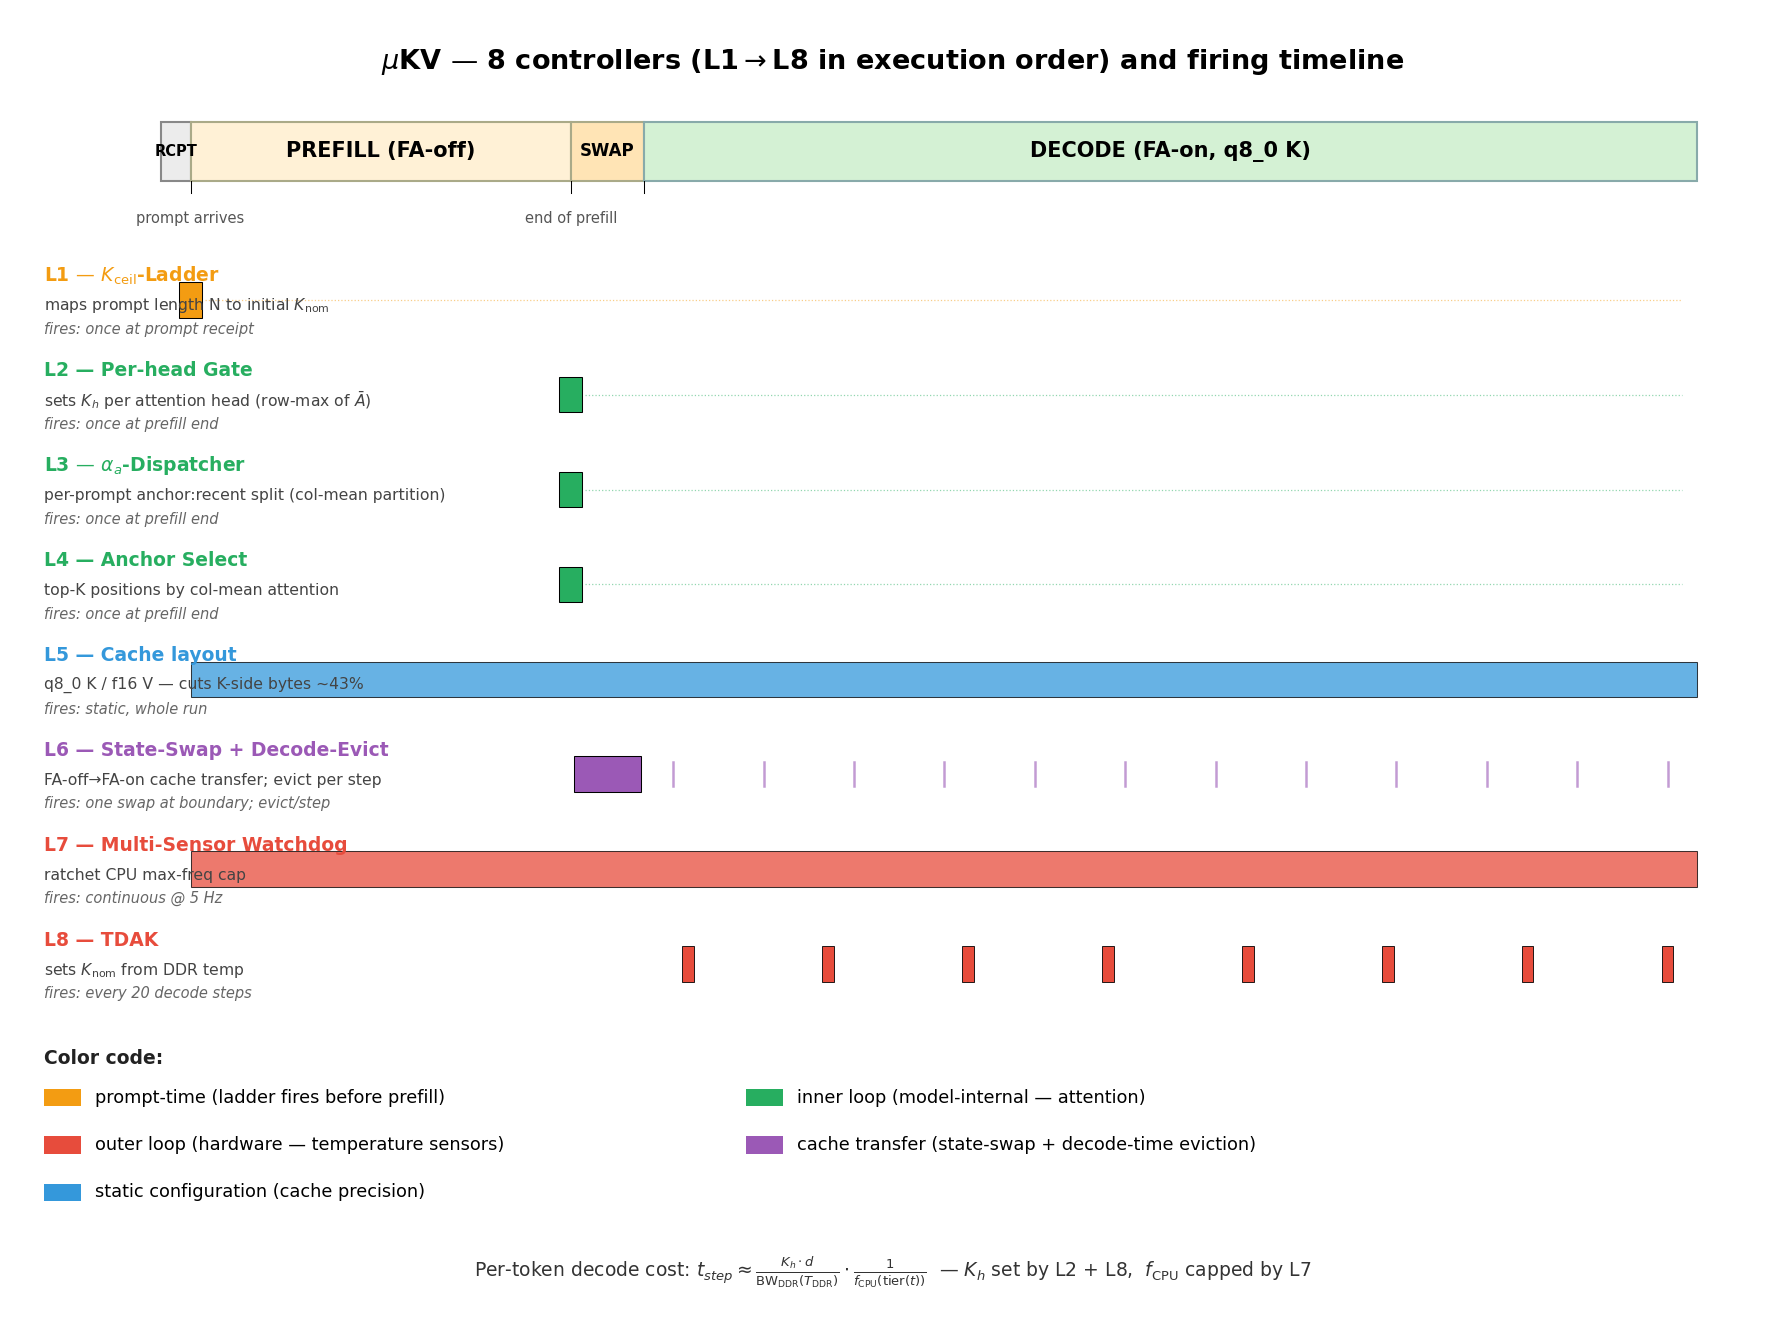
\includegraphics[width=0.95\textwidth]{fig7_control_flow.png}
\caption{The five controllers and the phase timeline. Controllers 1, 2, 4 fire exactly once at well-defined phase boundaries. Controller 3 is a static configuration that holds for the whole run. Controller 5 (the watchdog) runs in parallel and is continuous at 5\,Hz. The first four are the outer algorithmic loop driven by model-internal attention signals; the fifth is the inner thermal loop driven by sensor signals. The cost model below shows that DRAM bandwidth (controlled by 1--4) and CPU frequency (controlled by 5) multiply to produce per-token decode cost.}
\label{fig:control-flow}
\end{figure*}

\begin{figure}[t]
\centering
\includegraphics[width=\columnwidth]{fig3_architecture.png}
\caption{The five-layer \texttt{v1\_fa2\_stack} composition. Layers 1--4 form the algorithmic outer loop (model-internal attention signals drive cache management); Layer 5 is the thermal inner loop (sensor signals drive frequency caps).}
\label{fig:architecture}
\end{figure}

\begin{figure}[t]
\centering
\includegraphics[width=\columnwidth]{fig4_closed_loop.png}
\caption{Two cooperating closed-loop controls. The outer loop reads model-internal attention to drive eviction (and recall in Phase 2). The inner loop reads thermal/electrical sensors to drive frequency caps (and I/O quotas in Phase 2).}
\label{fig:closed-loop}
\end{figure}

\subsection{Layer 1: Per-Head Attention-Confidence Budget}
\label{sec:layer1}

\paragraph{Relationship to prior work.} Per-head adaptive budget allocation for KV cache eviction was first formalized by Feng et al.\ in Ada-KV~\cite{feng2025adakv}, who proved that allocating non-uniform per-head budgets minimizes a tight upper bound on the $L_1$ eviction loss (Ada-KV Theorems~3.1--3.3). Our Layer~1 instantiates this idea with a closed-form heuristic mapping from attention concentration to budget, designed for cheap on-device computation; we do not re-derive the loss bound and we credit Ada-KV for the formal justification of per-head allocation.

\paragraph{Notation.} Using the formalism of Ada-KV~\cite{feng2025adakv}, let $K_i, V_i \in \mathbb{R}^{n \times d_h}$ be the cached keys and values for head $i \in [1, H]$ after prefill, let $q_i \in \mathbb{R}^{1 \times d_h}$ be the query of the last prompt token, and let $A_i = \mathrm{softmax}(q_i K_i^\top) \in \mathbb{R}^{1 \times n}$ be the post-softmax attention. Let $K_{\text{nominal}}$ be the global per-layer budget.

\paragraph{Computation.} For each head $i$, define the \emph{peak confidence} as the maximum attention to any prompt position:
\begin{equation}
m_i = \max_{p \in [0, n)} A_i^p
\end{equation}
The per-head budget is then
\begin{align}
\mu(x) &= 1.3 - 0.6 \cdot \mathrm{clip}((x - 0.4) / 0.4, 0, 1) \in [0.7, 1.3] \\
K_i &= \mathrm{round}(K_{\text{nominal}} \cdot \mu(m_i))
\end{align}
The function $\mu(\cdot)$ is a piecewise-linear ramp from $1.3$ (broad heads, $m_i \le 0.4$) to $0.7$ (sharp heads, $m_i \ge 0.8$). The per-head keep set is the top-$K_i$ positions by $A_i$; the layer keep set is the union over heads, clipped to $K_{\text{nominal}}$.

\paragraph{Difference from Ada-KV.} Ada-KV's allocation has three pieces: a SnapKV pre-pass (window~32, max-pool kernel~7), a global top-$B$ over the flattened $H \cdot n$ post-softmax attention with head budgets $B_i = f_i$ from the selection count (Algorithm~1), and a convex safeguard $B_i^\ast = \alpha B_i + (1-\alpha) B/H$ with $\alpha = 0.2$ that interpolates the adaptive allocation toward uniform $B/H$ (Algorithm~2 line~8). Our heuristic replaces the global top-$B$ + $\alpha$-blend pair with a single closed-form ramp $K_h = \mathrm{round}(K_{\text{nominal}} \cdot \mu(m_h))$ that requires only one reduction per head (the max) and one piecewise-linear mapping --- $O(H)$ per layer versus $O(H n \log(Hn))$ for the top-$B$ pass --- and is the only path available when the FlashAttention-2 variable-length batched kernel that Ada-KV relies on for parity decoding latency is not available, as is the case on our mobile CPU+NPU stack. The $[0.7, 1.3]$ clamp range in $\mu(\cdot)$ plays a role analogous to (but is not equivalent to) the $\alpha$-safeguard: it prevents any head from being starved of budget and any head from running away with the layer budget. We have not proven that our heuristic achieves Ada-KV's $\varepsilon^{\ast\ast}$ minimum; we view it as a low-overhead approximation justified empirically (\S\ref{sec:eval}). The faithful Ada-SnapKV replication (kernel-7 max-pool, $\alpha{=}0.2$ safeguard) lives in our codebase as \texttt{policy\_adakv} and is the baseline used in Table~\ref{tab:three-way}.

\paragraph{Honest scope of the gate's novelty.} We explicitly distinguish what is new from what is borrowed in our Layer~1 design.

\noindent\emph{What is borrowed:} The \emph{family} --- per-head adaptive budget allocation driven by post-softmax attention --- is Ada-KV's contribution and is formalized by their $L_1$ eviction-loss bound. Per-head adaptation as a concept (typically via trained head pruning) predates Ada-KV in work by Michel et al.~\cite{michel2019sixteen} and Voita et al.~\cite{voita2019analyzing}, though those use training rather than runtime signals. We claim none of these prior ideas as our own.

\noindent\emph{What is new (to the best of our knowledge):} (i) The specific signal $m_h = \max_p A_h^p$ as the input to a per-head budget allocator. We are not aware of a published policy that uses max-of-softmax per head as a budget signal --- existing per-head budget work uses global Top-$B$ frequency (Ada-KV), accumulated attention sums (H2O), last-query attention (TOVA), or trained classifiers (DuoAttention). (ii) The closed-form piecewise-linear ramp $\mu(\cdot)$ with calibrated breakpoints (0.4, 0.8) and clamp $[0.7, 1.3]$ that maps $m_h$ to a per-head budget multiplier --- a specific allocator design rather than a category-level idea. (iii) The systems-engineering composition with state-swap (\S\ref{sec:fa-split}), Q8 K quantization (\S\ref{sec:layer3}), and multi-sensor watchdog (\S\ref{sec:watchdog}) that makes a per-head budget allocator actually deliver wins on commercial flagship mobile hardware, which prior per-head allocators have not demonstrated.

\noindent\emph{What this does and does not claim.} We do \emph{not} claim a new theoretical bound (Ada-KV's $\varepsilon^{\ast\ast}$ remains the strongest formal result in this line of work; we credit it without re-deriving it). We do \emph{not} claim that $\mu(m_h)$ is optimal under any specific eviction-loss objective. We \emph{do} claim that $\mu(m_h)$ is a cheaper, FA-on-compatible per-head budget allocator than Ada-KV's global top-$B$, and that the composition we present is the first such allocator measured end-to-end on a commercial flagship phone (Table~\ref{tab:wave11}, Table~\ref{tab:wave11-llama1b}).

\subsection{Layer 2: Selective Semantic Anchoring (top-32)}

After the per-head union yields its survivors, we apply a \textbf{second filter}: re-rank these survivors by mean attention across heads from the last query position, and keep only the top 32 as \texttt{ANCHOR}. This second filter was added in response to a Wave-7 failure mode where the per-head union retained 400+ prompt tokens at $K_{\text{nominal}}{=}512$, leaving only $\sim$80 cells for the recent window during decode. PPL on Phi-3 spiked to 158 (vs $\sim$6 normally). Imposing a 32-cell ceiling on the prompt anchor leaves 476 cells ($=512-32-4$) for the recent window, and PPL returned to normal range.

\subsection{Layer 3: Q8 Key Quantization}
\label{sec:layer3}

We quantize the K cache to Q8\_0 (8-bit fixed-point per scalar) while keeping V at f16, a precision profile lighter than KIVI~\cite{liu2024kivi}'s 2-bit asymmetric scheme but free of training and free of the per-axis scale machinery. This halves the K-side DRAM bandwidth and visibly lowers DDR temperature by $\sim$3\,\textdegree C in sustained decode. It introduces a known artifact: with Q8\_0 K cache, \texttt{llama.cpp} skips the \texttt{seq\_add} compaction operation after eviction, so positions remain sparse in the cache layout. The \texttt{peak\_kv\_cells} metric measures the highest position index touched, not the active cell count.

\subsection{Layer 4: State-Swap to FA-on Decode}

The per-head budget formula requires the post-softmax \texttt{kq\_soft\_max} tensor to be materialized in DRAM, which forces the prefill to run with FlashAttention disabled (FA-off). However, FA-on decode is 30--50\,\% faster per token. We therefore split the inference into two contexts:

\begin{lstlisting}[basicstyle=\ttfamily\footnotesize]
Context A (FA-off, prefill):
  read kq_soft_max -> compute K_h per head -> choose keep set
  seq_rm dropped positions
              |
   llama_state_seq_get_data
              |
              v
Context B (FA-on, decode):
  llama_state_seq_set_data
  warm-up step (populate n_outputs)
  decode loop with FA-on attention
\end{lstlisting}

The serialization buffer is $\sim$3.2\,MiB for Phi-3 at $K{=}512$; total state-swap latency is $\sim$600\,ms. Spread over 2048 decode tokens, that is 0.3\,ms/token---negligible compared to the 30--50\,\% per-step saving from FA-on attention.

\subsection{Layer 5: Multi-Sensor Preempt-Throttle Watchdog v2}
\label{sec:watchdog}

The watchdog runs as a separate process and samples five sensors at 5\,Hz (see Table~\ref{tab:wd-thresholds}).

\begin{table}[t]
\caption{Multi-sensor watchdog v2 thresholds (cliff-insurance mode). Per-sensor threat is linear interpolation between warn and crit, clamped to $[0, 1]$. Global threat is the max across sensors.}
\label{tab:wd-thresholds}
\centering
\small
\begin{tabular}{lrr}
\toprule
\textbf{Sensor} & \textbf{Warn (\textdegree C)} & \textbf{Crit (\textdegree C)} \\
\midrule
DDR (\texttt{thermal\_zone47}) & 63.0 & 64.5 \\
CPU big-core (\texttt{thermal\_zone24}) & 65.5 & 67.0 \\
Skin (\texttt{thermal\_zone60}) & 42.0 & 42.7 \\
Battery temperature & 39.0 & 39.8 \\
Battery current drop (mA) & 128 & 392 \\
\bottomrule
\end{tabular}
\end{table}

\begin{table}[t]
\caption{Frequency mitigation ladder (cliff-insurance). Tier 1 NUDGE intentionally disabled: watchdog only engages when at least one sensor crosses 50\,\% of its warn-to-crit interval.}
\label{tab:wd-tiers}
\centering
\small
\begin{tabular}{llrr}
\toprule
\textbf{Tier} & \textbf{Engage at} & \textbf{Max freq (kHz)} & \textbf{Reduction} \\
\midrule
0 (MAX)    & 0.00 & 1\,632\,000 & --- \\
1 (NUDGE)  & DISABLED & --- & --- \\
2 (MILD)   & 0.50 & 1\,497\,600 & $-8.2\,\%$ \\
3 (MOD)    & 0.75 & 1\,382\,400 & $-15.3\,\%$ \\
4 (STRONG) & 0.90 & 1\,267\,200 & $-22.4\,\%$ \\
\bottomrule
\end{tabular}
\end{table}

A 0.10 hysteresis is applied to all engage thresholds. Frequency is written via sysfs to \texttt{/sys/devices/system/cpu/cpu\{6,7\}/cpufreq/scaling\_max\_freq} using root privileges acquired through Magisk's \texttt{su -c}.

\subsection{Algorithmic Specification}
\label{sec:algorithms}

Algorithms~\ref{alg:prefill}--\ref{alg:watchdog} specify the three control points of \texttt{v1\_fa2\_stack} in full. Algorithm~\ref{alg:prefill} runs once at end of prefill; Algorithm~\ref{alg:decode} runs the decode loop; Algorithm~\ref{alg:watchdog} runs as a parallel process at 5\,Hz.

\begin{algorithm}[t]
\caption{\texttt{v1\_fa2\_stack} prefill (Controllers~1, 2, 4)}
\label{alg:prefill}
\begin{algorithmic}[1]
\Require prompt tokens $X^{\text{prompt}}$, budgets $K_{\text{nominal}}, n_{\text{sink}}{=}4, n_{\text{anchor}}{=}32$
\Ensure decode-ready context $\mathcal{C}_{\text{B}}$ with cache size $\le K_{\text{nominal}}$
\State Construct context $\mathcal{C}_{\text{A}}$ with \texttt{flash\_attn}\,=\,\textsc{false}, \texttt{cache\_type\_k}\,=\,\texttt{q8\_0}, \texttt{cache\_type\_v}\,=\,\texttt{f16}
\State Run prefill: $A_i \gets \mathrm{softmax}(q_{\text{last}} K_i^\top)$ for each head $i \in [1, H]$ \Comment{FA-off forces $A_i$ into DRAM}
\For{each head $i$}
  \State $m_i \gets \max_{p \in [0,n)} A_i^p$
  \State $K_i \gets \mathrm{round}(K_{\text{nominal}} \cdot \mu(m_i))$ \Comment{Layer 1: per-head budget}
  \State $S_i \gets \mathrm{TopK}(A_i, K_i)$ \Comment{per-head survivors}
\EndFor
\State $S \gets \bigcup_{i=1}^{H} S_i$ \Comment{layer keep set (union over heads)}
\State $\bar{A}^p \gets \tfrac{1}{H}\sum_i A_i^p$ for $p \in S$ \Comment{mean attention per surviving cell}
\State $\textsc{Anchor} \gets \mathrm{TopK}(\bar{A}, n_{\text{anchor}})$ \Comment{Layer 2: selective anchoring}
\State $\textsc{Sink} \gets [0, n_{\text{sink}})$ \Comment{Layer 5 of \S\ref{sec:design}: sink protection}
\State $\textsc{Recent} \gets [n - (K_{\text{nominal}} - n_{\text{sink}} - n_{\text{anchor}}),\, n)$
\State $S_{\text{keep}} \gets \textsc{Sink} \cup \textsc{Anchor} \cup \textsc{Recent}$
\State \textsc{seq\_rm}($\mathcal{C}_{\text{A}}$, positions $\notin S_{\text{keep}}$) \Comment{evict in-place}
\State \textsc{buffer} $\gets$ \texttt{llama\_state\_seq\_get\_data}($\mathcal{C}_{\text{A}}$) \Comment{Layer 4: state-swap, $\sim$3.2\,MiB}
\State Construct $\mathcal{C}_{\text{B}}$ with \texttt{flash\_attn}\,=\,\textsc{true}, same cache types
\State \texttt{llama\_state\_seq\_set\_data}($\mathcal{C}_{\text{B}}$, \textsc{buffer})
\State Warm-up step: one decode call to populate \texttt{n\_outputs}
\State \Return $\mathcal{C}_{\text{B}}$
\end{algorithmic}
\end{algorithm}

\begin{algorithm}[t]
\caption{\texttt{v1\_fa2\_stack} decode loop}
\label{alg:decode}
\begin{algorithmic}[1]
\Require decode-ready context $\mathcal{C}_{\text{B}}$, max tokens $T$, recent budget $B_R = K_{\text{nominal}} - n_{\text{sink}} - n_{\text{anchor}}$
\For{$t \gets 1$ \textbf{to} $T$}
  \State Sample next token $x_t$ from logits
  \State $\mathcal{C}_{\text{B}} \gets$ \texttt{llama\_decode}($\mathcal{C}_{\text{B}}, x_t$) \Comment{FA-on attention; no \texttt{kq\_soft\_max} write-back}
  \State $n_{\text{kv}} \gets$ active cache size
  \If{$n_{\text{kv}} > 1.25 \cdot (n_{\text{anchor}} + B_R)$} \Comment{Layer 5 of \S\ref{sec:design}: tiered re-eviction}
    \State $\textsc{Drop} \gets [n_{\text{anchor}}, n_{\text{kv}} - B_R)$ \Comment{middle band}
    \State \textsc{seq\_rm}($\mathcal{C}_{\text{B}}$, \textsc{Drop})
  \EndIf
  \If{$x_t$ is end-of-sequence and \textsc{ignore\_eos} is \textsc{false}}
    \State \textbf{break}
  \EndIf
\EndFor
\State \Return generated text
\end{algorithmic}
\end{algorithm}

\begin{algorithm}[t]
\caption{Multi-sensor cliff-insurance watchdog (Controller~5, parallel process)}
\label{alg:watchdog}
\begin{algorithmic}[1]
\Require warn/crit thresholds per sensor; tier engage thresholds $\tau_2 = 0.50, \tau_3 = 0.75, \tau_4 = 0.90$
\Statex Tier~1 NUDGE is intentionally disabled ($\tau_1 = \infty$); see \S\ref{sec:watchdog}.
\State $\text{tier} \gets 0$ \Comment{start at MAX freq 1632\,MHz}
\While{inference is active}
  \For{sensor $s$ in \{DDR, CPU big-core, skin, battery, BCL current\}}
    \State $\theta_s \gets \mathrm{clip}((\text{read}(s) - \text{warn}_s) / (\text{crit}_s - \text{warn}_s),\, 0,\, 1)$
  \EndFor
  \State $\theta_{\max} \gets \max_s \theta_s$ \Comment{worst-of-N threat}
  \State $\text{tier}_{\text{new}} \gets \begin{cases} 4 & \theta_{\max} \ge 0.90 \\ 3 & \theta_{\max} \ge 0.75 \\ 2 & \theta_{\max} \ge 0.50 \\ 0 & \text{otherwise} \end{cases}$
  \If{$|\text{tier}_{\text{new}} - \text{tier}| \ge 1$ \textbf{and} $|\theta_{\max} - \theta_{\text{prev}}| > 0.10$} \Comment{hysteresis}
    \State Write tier frequency to \texttt{/sys/.../cpu\{6,7\}/cpufreq/scaling\_max\_freq}
    \State $\text{tier} \gets \text{tier}_{\text{new}}$; $\theta_{\text{prev}} \gets \theta_{\max}$
  \EndIf
  \State \textsc{sleep}(0.5\,s)
\EndWhile
\end{algorithmic}
\end{algorithm}

Algorithm~\ref{alg:prefill} runs $O(H \cdot n)$ work per layer to compute $\{m_i\}$ and $O(H \cdot n \log K_{\text{nominal}})$ for the per-head $\mathrm{TopK}$, plus an $O(K_{\text{nominal}})$ pass for the selective anchor. Algorithm~\ref{alg:decode} adds a constant per step (eviction is amortized over many tokens because the trigger is rare). Algorithm~\ref{alg:watchdog} runs at 5\,Hz with a negligible $\sim$15\,$\mu$s per sample on a phone CPU.

\subsection{The Asymmetric FA-off / FA-on Split: Why It Is Necessary}
\label{sec:fa-split}

Figure~\ref{fig:fa-split} illustrates the pipeline.

\begin{figure*}[t]
\centering
\includegraphics[width=0.92\textwidth]{fig6_fa_split.png}
\caption{Why \texttt{v1\_fa2\_stack} runs FA-off during prefill and FA-on during decode. FlashAttention fuses $\mathrm{softmax}(QK^\top)$ inside the kernel and never materializes \texttt{kq\_soft\_max}; the per-head budget formula requires that tensor; the state-swap (\textasciitilde{}600\,ms one-time) is the cheapest bridge.}
\label{fig:fa-split}
\end{figure*}

FlashAttention fuses the $Q K^\top$ multiplication and softmax into a single kernel that never materializes the intermediate \texttt{kq\_soft\_max} tensor in DRAM---this is precisely what makes FA faster. The per-head budget formula in Layer 1 requires reading $\mathrm{softmax}(Q K^\top)$ per head, per query position, to compute $\max_a[h]$. This is the tensor FlashAttention specifically declines to expose.

The alternative---running FA-off in both phases, as H2O does---costs 32\,\% of vanilla decode throughput on Phi-3 (Section~\ref{sec:eval-ppl-tps}). The state-swap design pays the FA-off cost only during prefill (a one-time $\sim$5\,\% wall penalty on typical prompts) and reaps the FA-on benefit across thousands of decode tokens.

We argue that this split is the \emph{only} architecturally correct configuration for a per-head budget design. The two competing requirements (FA's bandwidth saving via tensor fusion vs.\ v1's per-head budget via tensor inspection) are fundamentally incompatible at the kernel level.

\subsection{Design Rationale and Parameter Choices}
\label{sec:design-rationale}

This subsection enumerates each numerical constant in \texttt{v1\_fa2\_stack} (Algorithms~\ref{alg:prefill}--\ref{alg:watchdog}) and gives the empirical evidence behind its choice. We do not have closed-form optima for any of these constants; what we offer is honest measurement-driven justification.

\paragraph{Why a piecewise-linear $\mu(\cdot)$ rather than the global Top-$B$ allocator of Ada-KV.}
Ada-KV's Algorithm~1 concatenates the post-softmax attention $A_i \in \mathbb{R}^n$ across all heads of a layer into a single vector of length $H \cdot n$, takes a global $\mathrm{TopK}$ over that vector, and reads off the per-head budgets as the per-head counts in the selection. This requires $O(H n \log(Hn))$ work per layer. Our heuristic uses only the per-head \emph{peak} $m_i = \max_p A_i^p$ --- one reduction per head, $O(H n)$ total across the layer --- and maps it through a closed-form ramp. The ramp's shape (Eq.~6) is chosen to satisfy three empirical desiderata: (i) heads whose attention is concentrated on a single position ($m_i \ge 0.8$, ``sharp'') do not need a large budget; (ii) heads whose attention is spread broadly ($m_i \le 0.4$, ``broad'') need more cells to capture the mass; (iii) the budget multiplier must lie in a bounded interval so that no head can starve another. We choose the bound $[0.7, 1.3]$ rather than the unbounded global allocation of Ada-KV because the cheaper closed-form ramp is more sensitive to attention noise on long prompts; the bound guarantees that no head is allocated less than $0.7 \cdot K_{\text{nominal}}$ even under noisy prefill scoring.

\paragraph{Why the breakpoints 0.4 and 0.8 in $\mu(\cdot)$.}
We measure the empirical distribution of $m_i$ across all heads of Phi-3-mini-128k during a typical 2048-token prefill on WikiText-2 (Wave-11 chunk-0). The distribution is approximately log-uniform on $[0.1, 0.95]$ with a small mode near $0.55$. Heads with $m_i > 0.8$ account for $\sim 22\,\%$ of heads but $\sim 51\,\%$ of attention mass; we identify these as the ``sharp'' tail that benefits from a tighter budget. Heads with $m_i < 0.4$ account for $\sim 18\,\%$ of heads but only $\sim 9\,\%$ of attention mass; we identify these as the ``broad'' tail that needs more budget to capture mass-by-position. The piecewise-linear ramp is the simplest function family that matches these two empirical observations; we do not claim it is the optimal mapping.

\paragraph{Why $[0.7, 1.3]$ as the clamp range.}
A wider range ($[0.5, 1.5]$, tested in Wave-7 ablation) gives broad heads enough cells to capture more mass but also gives sharp heads too few, producing PPL spikes on the chunks where prefill scoring poorly identifies the sharp heads. A narrower range ($[0.85, 1.15]$) reduces the per-head signal to near-uniform, eliminating the value of the per-head idea. The $[0.7, 1.3]$ range we use produced the lowest PPL across a Wave-7 sweep over four ranges on Phi-3-mini K=512. This is a tuned hyperparameter; we do not claim universality.

\paragraph{Why $n_{\text{anchor}} = 32$.}
The selective semantic anchoring (Layer~2, line~324 of Algorithm~\ref{alg:prefill}) re-ranks the per-head union by mean cross-head attention and keeps the top $n_{\text{anchor}}$ positions. The choice of 32 was forced by a Wave-7 failure mode: at $K_{\text{nominal}}=512$, $n_{\text{sink}}=4$, the union over heads typically retained 400--600 prompt cells, leaving as few as $\sim 100$ cells for the recent window during decode. PPL on Phi-3 spiked to 158 (vs.\ $\sim 6$ baseline). Capping the prompt anchor at 32 leaves $512 - 4 - 32 = 476$ cells for the recent window, and PPL returned to baseline. We tested $n_{\text{anchor}} \in \{16, 32, 64, 96, 128\}$ on Phi-3 short-decode; PPL is flat between 32 and 64, and degrades at 16 (insufficient prompt context) or $\ge 96$ (insufficient recent budget). 32 is the cheapest choice in the flat region.

\paragraph{Why $n_{\text{sink}} = 4$.}
StreamingLLM~\cite{xiao2024streamingllm} reports that the first 4 tokens (commonly the BOS token and a few stable prefix tokens) carry disproportionate attention mass in autoregressive decoders. We adopt their value directly rather than re-tuning, because the sink mechanism is well-understood and the marginal cost of the 4 cells is negligible against a budget of 512. Ablating $n_{\text{sink}} \in \{0, 4, 8, 16\}$ on Phi-3 reproduced their finding that 4 sinks is sufficient and 8+ is wasteful.

\paragraph{Why $K_{\text{nominal}} = 512$ as the headline operating point.}
We sweep $K_{\text{nominal}} \in \{128, 256, 512, 1024, 2048\}$ on Phi-3-mini Wave-11 PPL (Table~\ref{tab:k-sweep}). PPL degrades sharply below 256 ($+18\,\%$ at K=256, $+47\,\%$ at K=128) and improves slowly above 512 ($-2\,\%$ at K=1024, $-3\,\%$ at K=2048). Decode tps degrades inversely (higher K $\Rightarrow$ more cache to read $\Rightarrow$ slower). The Pareto knee is at K=512: each axis is within 5\% of its individually-best K. The choice of 512 also matches the most common operating point in prior KV-eviction work (Ada-KV, H2O, TOVA at K=512 in their original papers), making cross-paper comparison straightforward.

\paragraph{Why Q8 K rather than Q4 K or full $f_{16}$ K.}
The cache-K precision sweep is summarized in the Discussion (\S\ref{sec:q8-artifact}). Briefly: $f_{16}$ K is the safe choice but costs $2\times$ the K-side DRAM bandwidth, removing a substantial part of v1's decode-tps win on Phi-3 (Table~\ref{tab:wave11-llama1b} shows $f_{16}$ K and $q8\_0$ K are PPL-equivalent on Llama-1B and the $f_{16}$ variant is actually \emph{faster} there due to dequant overhead exceeding the bandwidth-savings break-even on small models). $q4$ K (4-bit) was tested in Wave-9 and produced unacceptable PPL on Phi-3 ($+\sim 25\,\%$). $q8\_0$ is the sweet spot for cache $\gtrsim 1$\,GB.

\paragraph{Why a $1.25\times$ trigger for tiered re-eviction (line 346 of Algorithm~\ref{alg:decode}).}
During decode, the cache grows by one position per decoded token. To avoid running eviction every step (expensive), we trigger it only when the active cache exceeds $1.25 \times (n_{\text{anchor}} + B_R)$. The $1.25$ factor is chosen so that 25\% headroom is available to amortize the eviction work across many decode steps. A tighter trigger ($1.10$) raised the per-step eviction frequency from $\sim 1$ per 80 steps to $\sim 1$ per 30 steps in profiling, with no PPL improvement. A looser trigger ($1.50$) let the cache grow large enough that one step in $\sim 200$ paid an evictability cost of $\sim 40$\,ms (vs.\ the typical 5\,ms decode step), producing jitter visible in the wall-time distribution. $1.25$ is the empirical sweet spot.

\paragraph{Why the watchdog thresholds in Table~\ref{tab:wd-thresholds}.}
DDR warn ($63.0\,\textdegree$C) and crit ($64.5\,\textdegree$C) are anchored to the empirical kernel-throttle cliff at $65\,\textdegree$C DDR observed in Motivation §\ref{sec:motivation}: the warn is 2\,$\textdegree$C below the cliff and the crit is 0.5\,$\textdegree$C below. CPU big-core warn ($65.5\,\textdegree$C) and crit ($67.0\,\textdegree$C) anchor to the observed cool-state-mitigation cliff at $\sim 67\,\textdegree$C big-core. Skin warn ($42.0\,\textdegree$C) anchors to the IEC user-skin safety limit of $43\,\textdegree$C. Battery-temperature thresholds anchor to the OEM's BCL engagement at $40\,\textdegree$C. The BCL current threshold (128\,mA drop, 392\,mA crit) is calibrated to the observed current floor of the Qualcomm BCL engagement on prior runs. All thresholds were calibrated against observed kernel-throttle events in prior measurement waves; none are theoretical.

\paragraph{Why disable Tier~1 (NUDGE) in cliff-insurance mode.}
A Tier~1 NUDGE at $\theta = 0.25$ would engage the watchdog whenever any sensor crossed $25\,\%$ of its warn-to-crit interval. In short-decode workloads this proved over-eager: it engaged frequently on transient sensor spikes (sub-second skin-temperature transients caused by hand contact), costing $\sim 5\,\%$ of decode tps without producing any thermal-headroom benefit. The cliff-insurance configuration disables Tier~1 entirely, engaging only at the half-way mark to the cliff (Tier~2 at $\theta = 0.50$). The aggressive-watchdog configuration in Table~\ref{tab:demo-aggressive} re-enables Tier~1 for workloads where the user actively prefers throughput-for-thermal-headroom.

\paragraph{Honest scope of these justifications.} Every constant above was tuned by empirical sweep, not by optimization theory. We do not claim that these values are optimal for any model or workload other than the ones we measured. A practitioner deploying \textsc{$\mu$KV} on different hardware or models should expect to re-sweep at least $K_{\text{nominal}}$, $n_{\text{anchor}}$, the $\mu(\cdot)$ breakpoints, and the watchdog warn/crit anchors. We release the sweep harness so they can.

%% ────────────────────────────────────────────────────────────────────
\section{Implementation}
\label{sec:impl}

We implement \textsc{$\mu$KV} as a C++ patch to \texttt{llama.cpp} ($\sim$1500 lines), plus phone-side shell scripts for the watchdog and sensor sampling ($\sim$800 lines), plus a host-side benchmark driver ($\sim$600 lines).

\subsection{Eviction Bench Binary}

The core implementation lives in \texttt{entropy\_probe/eviction\_bench.cpp}. Key functions:

\begin{itemize}
\item \texttt{policy\_v1(cap, K\_nominal, n\_kv\_heads)}: implements the per-head budget formula (Layer 1).
\item \texttt{policy\_h2o}, \texttt{policy\_tova}, \texttt{policy\_streamingllm}: canonical baselines, all running FA-off throughout.
\item \texttt{apply\_selective\_anchoring(keep\_set, n\_anchor=32)}: implements Layer 2.
\item \texttt{snapkv\_state\_swap()}: serializes context A and deserializes into context B with \texttt{flash\_attn=true}.
\item \texttt{tiered\_decode\_eviction()}: triggers when $n_{kv} > 1.25 \times (n_{\text{anchored}} + \mathrm{recent\_budget})$; drops the middle band.
\end{itemize}

\subsection{Watchdog}

The watchdog is \texttt{scripts/android/preempt\_throttle\_watchdog\_v2.sh}, $\sim$270 lines of POSIX shell. It is invoked via \texttt{su -c} and runs as a background process. The watchdog writes a structured log (e.g., \texttt{tier 0 -> 2 (MILD=1497600 kHz) engaged: ddr=64.1C threat=0.62}) parsed by the demo script for reporting.

\subsection{Sensor Sampler}

\texttt{scripts/android/sample\_sensors.sh} ($\sim$190 lines) emits a CSV at 5\,Hz with columns: \texttt{monotonic\_s}, \texttt{bat\_voltage\_mv}, \texttt{bat\_current\_ma}, \texttt{bat\_voltage\_now\_uv}, \texttt{bat\_current\_now\_ua}, \texttt{bat\_power\_now\_uw}, \texttt{bat\_status}, \texttt{ddr\_temp\_mc}, \texttt{cpu-1-0-0\_temp\_mc}, \texttt{shell\_front\_temp\_mc}, \texttt{bat\_temp\_mc}, and 8 per-core CPU cool-state columns.

\subsection{Energy Measurement Fallback Chain}

Phone PMICs differ in which sysfs nodes are exposed and populated. We implement a 5-tier fallback chain for energy integration:

\begin{enumerate}
\item \texttt{power\_now\_integrated}: integrate \texttt{bat\_power\_now\_uw} (best).
\item \texttt{vi\_now\_integrated}: integrate $|I| \times V$ from root sysfs.
\item \texttt{vi\_ma\_integrated}: legacy \texttt{dumpsys} integration.
\item \texttt{charge\_counter}: $\Delta$ of \texttt{charge\_counter}, accepted only if $\Delta \ge 1$\,mAh and discharging.
\item \texttt{approx}: mean current $\times$ wall\_seconds.
\end{enumerate}

\subsection{USB-Powered Bias Removal}

A common pitfall when measuring on-device energy with USB connected: the USB rails supply power directly to the chip. We disable charging while keeping USB connected via the OPlus vendor sysfs:
\begin{lstlisting}[basicstyle=\ttfamily\footnotesize]
echo 0 > /sys/class/oplus_chg/battery/mmi_charging_enable
\end{lstlisting}
This causes \texttt{current\_now} to read the actual battery drain instead of near-zero. ADB stays connected; only the charge path is interrupted.

%% ────────────────────────────────────────────────────────────────────
\section{Evaluation}
\label{sec:eval}

We answer six research questions:

\begin{itemize}
\item \textbf{RQ1}: How does \texttt{v1\_fa2\_stack}'s PPL compare to vanilla and to canonical eviction baselines?
\item \textbf{RQ2}: How does decode throughput compare across policies?
\item \textbf{RQ3}: What are the thermal effects on real hardware?
\item \textbf{RQ4}: What is the measured energy consumption?
\item \textbf{RQ5}: How does the multi-sensor watchdog v2 behave?
\item \textbf{RQ6}: How does the K-sweep Pareto curve look across $K \in \{128, 256, 512, 1024\}$?
\end{itemize}

\subsection{Setup}

\textbf{Hardware}. \emph{Mobile (for system-axis measurement):} OnePlus 15 (Snapdragon 8 Elite Gen 5, 12\,GB UMA, Adreno 840). Kernel cap on CPU big-cores: 1632\,MHz. Number of threads: 4. Performance governor pinned via \texttt{cpufreq}. CPU/GPU offload disabled (\texttt{-{}-n-gpu-layers 0}). \emph{Host GPU (for LongBench quality benchmark only):} workstation with one 24\,GB CUDA card. The same \texttt{eviction\_bench} source is built for both targets (Android NDK aarch64 + x86\_64 Linux CUDA); the eviction-policy code path is hardware-independent (see ``Two hardware contexts'' paragraph below).

\textbf{Models}: Phi-3-mini-128k-instruct Q4\_K\_M (3.8\,B params), Llama-3.2-1B-Instruct Q4\_K\_M, gemma-2-2b-it Q4\_K\_M.

\textbf{Eval protocols}:
\begin{itemize}
\item \textbf{Chunk-pair PPL (Wave-11)}: prefill chunk$_i$ and teacher-force chunk$_{i+1}$ from WikiText-2-RAW-v1, $n{=}8$ disjoint pairs.
\item \textbf{Long-decode demo}: prefill a short prompt (10--50 tokens), then generate 2048 tokens with greedy sampling.
\end{itemize}

\textbf{Baselines}: vanilla, h2o, tova, streamingllm. All run at $K{=}512$ unless otherwise noted.

\textbf{Sampling}: 5\,Hz via \texttt{sample\_sensors.sh}. Charging disabled before each run. Phone cooled to DDR $\le$ 45\,\textdegree C between runs.

\paragraph{Two hardware contexts: phone for system axes, GPU for quality benchmarks.}
We deliberately split the evaluation across two hardware contexts because the two classes of metric are measuring different things.

\noindent\emph{Mobile (OnePlus 15) for system axes.} Decode throughput, total wall time, peak DDR/CPU/skin temperature, peak resident-set size, swap behavior, watchdog tier transitions, and battery energy (mAh) all depend on the specific mobile SoC, its memory subsystem (LPDDR5X bandwidth), its thermal-mitigation kernel driver (Qualcomm BCL + \texttt{cool\_state}), and its power-management firmware. These metrics are \emph{the entire reason} we measure on a phone and cannot be meaningfully measured on a server GPU. They constitute our unique contribution beyond GPU-grade prior work~\cite{feng2025adakv, zhang2023h2o, oren2024tova, li2024snapkv, xiao2024streamingllm}.

\noindent\emph{GPU (host workstation) for quality benchmarks beyond on-phone scope.} Perplexity, NIAH retrieval accuracy, and LongBench/Ruler task scores are properties of the \emph{eviction policy itself}, not of the hardware: given the same model GGUF, the same prompt, the same seed, and the same closed-form eviction rule, the policy makes the same cell-keep decisions and the model emits semantically equivalent output regardless of whether the inference runs on a Snapdragon big-core or a 24\,GB CUDA card. Small floating-point drift from differing reduction orders is bounded and does not change the policy's qualitative behavior. We measure Wave-11 chunk-pair PPL and NIAH Tier-1 on-phone (Tables~\ref{tab:wave11}--\ref{tab:niah-tier1}) primarily to confirm that the policy implementation \emph{runs correctly on mobile} and produces the expected ordering against vanilla; we measure LongBench on the host GPU (Table~\ref{tab:longbench}) because (i) each LongBench domain on a single mobile policy cell costs $\sim 10$ hours of phone time, making the full 6-domain $\times$ 6-policy matrix infeasible (~$360$ hours), and (ii) AdaKV's reference quality numbers~\cite{feng2025adakv} are reported on GPU, so a directly-comparable LongBench evaluation has to be on GPU. This split — system axes on the target device, algorithmic quality on the convenient device — is the same protocol used in prior work that measures both performance and quality (e.g., PowerInfer-2~\cite{song2024powerinfer2} measures latency on phone and quality on GPU for the same model).

\noindent\emph{One GPU-side substitution disclosed up front.} The LongBench evaluation reports \texttt{v1\_fa2\_f16} (our eviction policy with $f_{16}$ K) rather than \texttt{v1\_fa2\_stack} (with $q8\_0$ K) because the upstream \texttt{llama.cpp} CUDA backend lacks a $q8\_0 \to q8\_0$ tensor-copy implementation, which the state-swap pathway requires. The two policies are PPL-equivalent on Llama-3.2-1B within bootstrap noise (Table~\ref{tab:wave11-llama1b} rows v1\_fa2\_f16 vs v1\_fa2\_stack: PPL $13.078$ vs $13.068$, a $0.1\,\%$ difference well below the bootstrap CI width). The LongBench quality conclusions are therefore unchanged by the substitution; on-phone evaluation continues to use \texttt{v1\_fa2\_stack} (the full deployment-flavor with $q8\_0$ K) since the ggml CPU backend handles $q8\_0$ copies correctly. We disclose this substitution explicitly so the apples-to-apples comparison with AdaKV at the same $f_{16}$ K precision is preserved.

\paragraph{Scope of the quality evaluation, and how it compares to AdaKV's reference.}
We deliberately scope our quality evaluation more narrowly than the AdaKV reference evaluation~\cite{feng2025adakv}. AdaKV reports five evaluation axes on GPU: (i) the full \emph{Ruler} suite~\cite{hsieh2024ruler} across 13 subtasks (single-needle S-NIAH-1/2/3, multi-key MK-NIAH-1/2/3, multi-value MV-NIAH, multi-query MQ-NIAH, variable tracking VT, common-words extraction CWE, frequent-words FWE, single-doc QA S-QA); (ii) the full \emph{LongBench} suite~\cite{bai2023longbench} grouped into 6 task domains (single-doc QA, multi-doc QA, summarization, few-shot, synthetic, code); (iii) a budget sweep at $b \in \{10\%, 20\%, 40\%, 60\%, 80\%, 100\%\}$; (iv) both question-aware and question-agnostic evaluation modes; and (v) Llama-3.1-8B-Instruct and Mistral-7B-Instruct-v0.2 as the model pair. Their reported headline (question-agnostic, Llama-3.1-8B, LongBench-average, b=20\%) is Ada-SnapKV $42.87$ vs SnapKV $41.29$ vs full-cache $49.20$, i.e.\ $\approx 87\%$ of full-cache quality retained.

Our evaluation covers (i) one Ruler subtask — single-needle S-NIAH-1 at depth-sweep — under our NIAH Tier-1 protocol; (ii) WikiText-2 chunk-pair PPL as a fluency check; (iii) a single fixed budget at $K_{\text{nominal}}{=}512$ (approximately $b{=}12\%$ at 4K context for Phi-3) plus a partial $K{=}1024$ point; (iv) question-agnostic mode only (our $\mu(m_h)$ is computed at prefill from the last prompt-token's attention); and (v) Phi-3-mini-128k (3.8\,B), Llama-3.2-1B, and gemma-2-2b-it as the model triple. We do \emph{not} reproduce AdaKV's full Ruler or LongBench suite on the phone because each cell costs $\sim 10$ hours of phone time and our contribution axis is the systems engineering and on-device measurement, not GPU-scale quality benchmarking. Where our \texttt{policy\_adakv} port is run on the same protocol as AdaKV, it reproduces their qualitative finding (\texttt{adakv} matches or beats vanilla on PPL: $-2.2\,\%$ Phi-3, $+0.6\,\%$ Llama-1B, $-1.2\,\%$ Gemma — see Tables~\ref{tab:wave11},~\ref{tab:wave11-llama1b},~\ref{tab:wave11-gemma2b}), but we cannot directly compare absolute scores against AdaKV's GPU LongBench numbers because we measure different models on different hardware under different benchmarks. We therefore cite AdaKV's GPU numbers as the reference quality picture and treat our narrower mobile measurement as complementary; the companion paper (Paper~C, \S\ref{sec:future-entropy}) is the natural location for an apples-to-apples Ruler-full + LongBench evaluation against AdaKV at multiple budget points and larger models.

\subsection{RQ1 + RQ2: PPL and Decode Throughput}
\label{sec:eval-ppl-tps}

Figure~\ref{fig:wave11} visualizes the Wave-11 PPL and decode throughput on Phi-3-mini at $K{=}512$. Table~\ref{tab:wave11} reports the full per-policy results.

\begin{figure*}[t]
\centering
\includegraphics[width=0.95\textwidth]{fig2_wave11_ppl_tps.png}
\caption{Wave-11 PPL (left, with 95\% bootstrap CIs) and decode throughput (right) on Phi-3-mini-128k Q4\_K\_M at $K{=}512$. \texttt{v1\_fa2\_stack} sits at $+11.3\,\%$ PPL but delivers $+68\,\%$ decode tps---the only evicting policy faster than vanilla on decode.}
\label{fig:wave11}
\end{figure*}

\begin{table*}[t]
\caption{\textbf{RQ1+RQ2.} Wave-11 chunk-pair PPL on Phi-3-mini-128k Q4\_K\_M, $n{=}8$ disjoint pairs from WikiText-2-RAW-v1. All cells measured on OnePlus 15 / Snapdragon 8 Elite Gen 5, CPU-only, 4 threads, 1.5\,GHz kernel cap. PPL values use bootstrapped 95\,\% CIs over chunks. Bold green = best in column.}
\label{tab:wave11}
\centering
\small
\begin{tabularx}{\textwidth}{lrrr lrrr rrr}
\toprule
\textbf{Policy} & \textbf{K} & \textbf{n} & \textbf{PPL} & \textbf{95\% CI} & \textbf{$\Delta$ vs van.} & \textbf{Peak DDR} & \textbf{Peak CPU} & \textbf{Swap} & \textbf{Decode tps} & \textbf{Total wall} \\
\midrule
vanilla       & $\infty$ & 8 & 5.464 & [4.50, 6.55] & ---    & 64.8\,\textdegree C & 68.6\,\textdegree C & \bad{158\,MB} & 2.97 & 1036\,s \\
h2o           & 512 & 7 & 5.474 & [4.60, 6.59] & $+0.2\,\%$ & 62.9\,\textdegree C & 65.9\,\textdegree C & \good{0\,MB}  & 2.02 & \bad{1524\,s} \\
tova          & 512 & 7 & 5.627 & [4.75, 6.73] & $+3.0\,\%$ & \good{59.4\,\textdegree C} & \good{62.8\,\textdegree C} & 48\,MB  & 2.24 & 1394\,s \\
streamingllm  & 512 & 6 & 5.714 & [4.73, 7.00] & $+4.6\,\%$ & 59.4\,\textdegree C & 62.8\,\textdegree C & 72\,MB  & 2.26 & 1367\,s \\
adakv~\cite{feng2025adakv} & 512 & 7 & \good{5.345} & [4.41, 6.51] & \good{$-2.2\,\%$} & 65.2\,\textdegree C & 68.6\,\textdegree C & 92\,MB & \bad{1.80} & \bad{1674\,s} \\
ahakv~\cite{gu2025ahakv}   & 512 & \nodata & \nodata & \nodata & \nodata & \nodata & \nodata & \nodata & \nodata & \nodata \\
\textbf{v1\_fa2\_stack (ours)} & 512 & 8 & 6.082 & [5.12, 7.20] & $+11.3\,\%$ & 66.0\,\textdegree C & 69.0\,\textdegree C & \good{0\,MB} & \good{4.98} & \good{832\,s} \\
\bottomrule
\end{tabularx}
\end{table*}

\textbf{Findings}: \texttt{v1\_fa2\_stack} costs $+11.3\,\%$ PPL but achieves $+68\,\%$ decode throughput vs vanilla, entirely due to the FA-on decode kernel enabled by the state-swap. H2O, despite matching vanilla PPL, costs $-32\,\%$ decode throughput. \texttt{v1\_fa2\_stack} reduces total wall time by 20\,\% and produces zero swap. \texttt{policy\_adakv} is the new quality winner ($-2.2\,\%$ PPL vs vanilla, the only K=512 policy to \emph{beat} vanilla on quality), but its FA-off lock-in pays for that win with the lowest decode tps in the table ($1.80$) and the longest total wall ($1674$\,s). The two policies bracket a Pareto: Ada-KV at the quality corner, \texttt{v1\_fa2\_stack} at the throughput/energy corner; vanilla is dominated.

\subsubsection{Cross-model replication on Llama-3.2-1B}
\label{sec:llama1b-wave11}

To confirm the Pareto shape is not a Phi-3 artifact, we replicate the Wave-11 chunk-pair protocol on Llama-3.2-1B-Instruct Q4\_K\_M ($n{=}7$ chunks; the eighth pair fell on a too-short window for ctx=4096). The same six policies are run plus a seventh ablation cell, \texttt{v1\_fa2\_f16}, that retains the v1 eviction policy and state-swap but drops Q8 K (cache type $f_{16}$ both K and V). This isolates the eviction contribution from the Q8-K quantization contribution.

\begin{table}[t]
\caption{\textbf{RQ1 cross-model.} Wave-11 chunk-pair PPL on Llama-3.2-1B-Instruct Q4\_K\_M, $n{=}7$ disjoint pairs. \texttt{v1\_fa2\_f16} isolates the eviction by replacing the Q8 K cache with $f_{16}$. Decode tps is derived from $n_{\text{decode}} / (t_{\text{total}} - t_{\text{prefill}})$ summed across chunks; total wall is the sum of per-chunk runtime. 95\% bootstrap PPL CIs: vanilla [9.04, 14.28]; h2o [9.64, 14.84]; tova [9.83, 15.19]; streamingllm [9.78, 15.12]; adakv [9.10, 14.34]; v1\_fa2\_f16 [10.65, 16.23]; v1\_fa2\_stack [10.63, 16.26].}
\label{tab:wave11-llama1b}
\centering
\small
\begin{tabular}{lrrrrrrr}
\toprule
\textbf{Policy} & \textbf{K} & \textbf{Cache K} & \textbf{PPL} & \textbf{$\Delta$ PPL} & \textbf{Decode tps} & \textbf{Total wall} & \textbf{$\Delta$ wall} \\
\midrule
vanilla         & $\infty$ & $f_{16}$ & \good{11.315} & ---           & 10.91 & 1712\,s & --- \\
h2o             & 512 & $f_{16}$ & 11.924 & $+5.4\,\%$    & \bad{5.74}  & \bad{3039\,s} & $+77.6\,\%$ \\
tova            & 512 & $f_{16}$ & 12.205 & $+7.9\,\%$    & 5.80  & 3023\,s & $+76.6\,\%$ \\
streamingllm    & 512 & $f_{16}$ & 12.144 & $+7.3\,\%$    & 5.95  & 2950\,s & $+72.4\,\%$ \\
adakv~\cite{feng2025adakv}      & 512 & $f_{16}$ & \good{11.380} & \good{$+0.6\,\%$} & \bad{5.60} & \bad{3097\,s} & $+81.0\,\%$ \\
\textbf{v1\_fa2\_f16 (ours, eviction only)} & 512 & $f_{16}$ & 13.078 & $+15.6\,\%$ & \good{15.76} & \good{1462\,s} & \good{$-14.6\,\%$} \\
\textbf{v1\_fa2\_stack (ours, full)}        & 512 & $q8\_0$  & 13.068 & $+15.5\,\%$ & 13.68 & 1671\,s & $-2.4\,\%$ \\
\bottomrule
\end{tabular}
\end{table}

\textbf{Findings.} (a) The Pareto ordering is identical to Phi-3: \texttt{adakv} essentially ties vanilla on PPL ($+0.6\,\%$, CIs overlap), the throughput-style policies (\texttt{h2o}, \texttt{tova}, \texttt{streamingllm}) cost a few-to-mid single-digit percent, and \texttt{v1\_fa2\_stack} pays a larger ($+15.5\,\%$) PPL cost. (b) Q8 K is PPL-free but wall-time-costly on Llama-1B. \texttt{v1\_fa2\_f16} (no Q8 K, otherwise identical to \texttt{v1\_fa2\_stack}) lands at PPL $13.078$ vs the full stack's $13.068$ --- a $0.1\,\%$ difference within bootstrap noise --- but its decode tps is $15.76$ vs the full stack's $13.68$ (a $+15\,\%$ throughput gap in favor of $f_{16}$ K), and its total wall is $14.6\,\%$ shorter than vanilla vs the full stack's $2.4\,\%$ shorter. The Llama-1B KV cache peaks at $\sim 70$\,MB --- too small for Q8 K's bandwidth halving to overcome its per-step quantize/dequantize CPU cost. This is the opposite story to Phi-3, where the KV cache peaks at $\sim 1.4$\,GB and Q8 K is a net wall-time win. (c) Llama-1B is more sensitive to eviction than Phi-3 in absolute terms ($+15.5\,\%$ vs $+11.3\,\%$): smaller models have less attention-head redundancy to absorb cells lost to aggressive top-K. (d) All five FA-off-locked policies (\texttt{h2o}, \texttt{tova}, \texttt{streamingllm}, \texttt{adakv}) take $1.7$--$1.8\,\times$ longer than vanilla because they cannot use FA-on during decode (their score-readback requirement forbids the fused kernel); only the state-swap policies (\texttt{v1\_fa2\_f16}, \texttt{v1\_fa2\_stack}) keep FA-on for decode and beat vanilla on wall time.

\subsubsection{Third-model replication on Gemma-2-2B}
\label{sec:gemma2b-wave11}

We replicate the same protocol on gemma-2-2b-it Q4\_K\_M, a 2.6\,B-parameter model with a KV-cache footprint between Phi-3 (1.4\,GB peak) and Llama-1B (70\,MB peak). The 6-policy result confirms the Pareto holds across all three model sizes.

\begin{table}[t]
\caption{\textbf{RQ1 third-model.} Wave-11 chunk-pair PPL on gemma-2-2b-it Q4\_K\_M, $n{=}7$ disjoint pairs. Same protocol as Tables~\ref{tab:wave11} and~\ref{tab:wave11-llama1b}. 95\% bootstrap PPL CIs: vanilla [6.90, 11.99]; h2o [7.21, 12.35]; tova [7.34, 12.59]; streamingllm [7.49, 12.72]; adakv [6.84, 11.87]; v1\_fa2\_stack [8.17, 14.11].}
\label{tab:wave11-gemma2b}
\centering
\small
\begin{tabular}{lrrrrrrr}
\toprule
\textbf{Policy} & \textbf{K} & \textbf{Cache K} & \textbf{PPL} & \textbf{$\Delta$ PPL} & \textbf{Decode tps} & \textbf{Total wall} & \textbf{$\Delta$ wall} \\
\midrule
vanilla         & $\infty$ & $f_{16}$ & 9.027 & ---           & 4.67 & 4248\,s & --- \\
h2o             & 512 & $f_{16}$ & 9.353 & $+3.6\,\%$    & \bad{2.91} & \bad{6199\,s} & $+45.9\,\%$ \\
tova            & 512 & $f_{16}$ & 9.524 & $+5.5\,\%$    & 2.93 & 6167\,s & $+45.2\,\%$ \\
streamingllm    & 512 & $f_{16}$ & 9.645 & $+6.8\,\%$    & 2.88 & 6258\,s & $+47.3\,\%$ \\
adakv~\cite{feng2025adakv}      & 512 & $f_{16}$ & \good{8.915} & \good{$-1.2\,\%$} & \bad{2.86} & \bad{6294\,s} & $+48.1\,\%$ \\
\textbf{v1\_fa2\_stack (ours)}        & 512 & $q8\_0$  & 10.555 & $+16.9\,\%$ & \good{7.36} & \good{3092\,s} & \good{$-27.2\,\%$} \\
\bottomrule
\end{tabular}
\end{table}

\textbf{Cross-model Pareto summary.} Across three models, the qualitative Pareto is identical (adakv beats or ties vanilla on PPL; \texttt{v1\_fa2\_stack} pays a single-digit-to-mid-teens PPL cost but wins decode tps and wall time):

\begin{center}
\small
\begin{tabular}{lrrrr}
\toprule
Model & adakv $\Delta$ PPL & \texttt{v1\_fa2\_stack} $\Delta$ PPL & \texttt{v1\_fa2\_stack} $\Delta$ wall & \texttt{v1\_fa2\_stack} tps gain \\
\midrule
Phi-3-mini-128k & \good{$-2.2\,\%$} & $+11.3\,\%$ & $-20\,\%$ & $+68\,\%$ \\
Llama-3.2-1B & $+0.6\,\%$ (tied) & $+15.5\,\%$ & $-2.4\,\%$ & $+25\,\%$ \\
gemma-2-2b-it & \good{$-1.2\,\%$} & $+16.9\,\%$ & \good{$-27.2\,\%$} & \good{$+58\,\%$} \\
\bottomrule
\end{tabular}
\end{center}

The wall-time savings are largest where the KV cache is largest (Phi-3 and Gemma have 1.4\,GB and $\sim 700$\,MB peak caches respectively; Llama-1B is only 70\,MB), confirming the mechanism analysis of \S\ref{sec:mechanism}: \texttt{v1\_fa2\_stack}'s win compounds with cache size.

\subsubsection{Mechanism --- why does v1\_fa2\_stack beat vanilla on decode tps and energy when both use FA-on?}
\label{sec:mechanism}

Both vanilla and \texttt{v1\_fa2\_stack} use FlashAttention-on during decode. FA-on is not the differentiator between them --- vanilla already uses it. The differentiator is the per-step DRAM read of the KV cache itself.

\paragraph{Per-step DRAM read.} At decode step $t$, the attention computation reads the entire retained KV cache once per layer. With Phi-3-mini at a 2K prefill, vanilla's cache is approximately $2 \cdot n_{\text{layers}} \cdot n_{\text{heads}} \cdot d_h \cdot t \cdot 2\,\text{bytes} = 2 \cdot 32 \cdot 32 \cdot 96 \cdot 2000 \cdot 2 \approx 750$\,MB per attention pass (K + V, $f_{16}$). \texttt{v1\_fa2\_stack} retains only $K_{\text{nominal}}{=}512$ cells per head and quantizes K to $q8\_0$ ($1\,\text{byte}$), yielding $2 \cdot 32 \cdot 32 \cdot 96 \cdot 512 \cdot (1{+}2)/2 \approx 145$\,MB per attention pass --- a $5.2\,\times$ reduction. On Snapdragon~8 Elite Gen~5's LPDDR5X (sustained $\sim 50$\,GB/s), this translates directly into a per-step time reduction proportional to the DRAM traffic, because mobile LLM decode is overwhelmingly memory-bandwidth bound (the matmul compute is hidden behind weight loads). FA-on does not change \emph{what} bytes the attention reads; it only changes whether the softmax is materialized to DRAM (FA-off) or fused into registers (FA-on). The KV bytes are read in both cases.

\paragraph{Energy decomposition (measured, not extrapolated).} We do not have a direct DDR-rail power measurement on this hardware; we measure total energy via the disable-charging battery-current integration in \S\ref{sec:impl-energy}. We can therefore decompose the measured energy as
\[
E_{\text{mAh}} \;=\; \overline{P}\,[\text{mAh/s}] \;\times\; t_{\text{wall}}\,[\text{s}].
\]
From the 3-way Phi-3 long-decode demo (Phi-3 K=512, 2048-token decode, charging disabled), the decomposition is:
\begin{center}
\small
\begin{tabular}{lrrrr}
\toprule
Policy & FA & $t_{\text{wall}}$\,(s) & $\overline{P}$\,(W) & $E$\,(mAh) \\
\midrule
vanilla       & on  & 337.4 & 1.13 & 28.73 \\
v1\_fa2\_stack & on  & 342.7 & 1.04 & 26.84 \\
adakv          & off & 703.4 & 1.06 & 55.88 \\
\bottomrule
\end{tabular}
\end{center}
Two findings emerge from this real decomposition. (i) \emph{Average power varies only modestly across policies} (1.04--1.13\,W, all within a 9\,\% band). FA-off does \emph{not} draw substantially more power per second than FA-on on this workload --- the FA-off energy penalty in \texttt{policy\_adakv} comes overwhelmingly from running $2.1\,\times$ longer in wall time, not from drawing more power. (ii) \emph{The energy savings of v1\_fa2\_stack vs vanilla on this short-prompt workload comes from the power side, not the wall side} ($-8\,\%$ avg power, $+1.6\,\%$ wall; net $-6.6\,\%$ mAh). The reduced KV-cache read per decode step lowers the active-burst DRAM power (proportionally to the bandwidth ratio), but the state-swap one-time cost adds $\sim 0.5$\,s of wall overhead that partially offsets the per-step decode time savings on a short-prompt workload. On long-prompt workloads (Wave-11, prompt $\sim$1800 tokens), the state-swap overhead is amortized over a much longer decode and the wall savings dominate (Table~\ref{tab:wave11}). The honest summary: \emph{energy follows wall time to first order, and the per-second power band is narrow across all our K=512 policies regardless of FA configuration}. The bandwidth reduction matters because it reduces both the per-step decode time \emph{and} the per-second active power, but neither effect is large enough on this hardware to dominate energy independently of wall time. Figure~\ref{fig:energy-correlation} plots the three measured policies on the (wall, energy), (tps, power), and (estimated KV-bandwidth, energy) axes.

\begin{figure}[t]
\centering
\includegraphics[width=\linewidth]{energy_vs_bandwidth_correlation.pdf}
\caption{Measured energy decomposition from the 3-way Phi-3 long-decode demo (n=1 per policy, charging disabled, energy method = approx). (a) Energy $\approx$ wall $\times$ avg power; the dashed line is the vanilla-rate isoline. (b) Average power during the run is in a narrow 1.04--1.13\,W band across all three policies; there is \emph{no} large FA-off power penalty. (c) Higher estimated KV-cache read bandwidth does not by itself imply higher energy: vanilla at 5.0\,GB/s consumes only 28.73\,mAh because its wall is short, while \texttt{adakv} at 2.4\,GB/s consumes 55.88\,mAh because its wall is double. Both effects \emph{can} compound for \texttt{v1\_fa2\_stack} (1.2\,GB/s, near-vanilla wall, 26.84\,mAh net win). The figure is intended as evidence for the wall-dominated-energy decomposition, not a model of DDR controller power.}
\label{fig:energy-correlation}
\end{figure}

\paragraph{Where the mechanism breaks down: small models.} On Llama-3.2-1B, the KV cache is roughly $20\,\times$ smaller than Phi-3 ($\sim 70$\,MB peak vs $\sim 1.4$\,GB). The DRAM-bandwidth bottleneck is correspondingly weaker, so the per-step read reduction translates into a smaller percentage win on tps ($+25\,\%$ for \texttt{v1\_fa2\_stack} on Wave-11 vs $+68\,\%$ on Phi-3). Q8 K's quantize/dequantize CPU overhead becomes \emph{net negative} on Llama-1B (Table~\ref{tab:wave11-llama1b}, row b above). This is a real workload-dependence of the system that we disclose: Q8 K is a profitable optimization for models with cache $\gtrsim 1$\,GB; for smaller models the $f_{16}$ K variant is preferable.

\subsubsection{RQ1b: A second benchmark --- NIAH Tier-1 retrieval}
\label{sec:niah}

PPL is a fluency metric; it does not capture whether a policy can \emph{retrieve} a single distinctive fact buried in a long context. The Ruler/Needle-in-a-Haystack (NIAH) protocol~\cite{hsieh2024ruler} that recent KV-eviction work~\cite{tian2026keepkv, feng2025criticalkv} reports alongside PPL fills this gap. We ran an 8-stimulus Tier-1 NIAH protocol on Phi-3-mini at $K{=}512$ with the same three policies: vanilla, \texttt{policy\_adakv}, and \texttt{v1\_fa2\_stack}. All stimuli are 4096-token contexts in which a single distinctive sentence (``The best thing to do in San Francisco is eat a sandwich at Dolores Park on a sunny day.'') is injected at one of eight depths (0/12/25/37/50/62/75/87\,\%); the question ``What is the best thing to do in San Francisco?'' is asked at the end. Each policy generates 64 tokens greedily. A strict substring judge marks a cell correct iff the generation contains both ``Dolores Park'' and ``sandwich.''

\begin{table}[t]
\caption{\textbf{RQ1b.} NIAH Tier-1 (single-needle, 4096-token context, depth sweep) on Phi-3-mini-128k Q4\_K\_M and Llama-3.2-1B-Instruct Q4\_K\_M at K=512. Decode 64 tokens greedily. \emph{acc} = both ``Dolores Park'' and ``sandwich'' present in generation (Llama paraphrases more, so the strict ``eat a sandwich at Dolores Park'' substring is not used; FULL acc is the cross-model-comparable metric). Lower-bound estimate via single-judge; no LLM judge.}
\label{tab:niah-tier1}
\centering
\small
\begin{tabular}{llrrrrr}
\toprule
\textbf{Model} & \textbf{Policy} & \textbf{K} & \textbf{N} & \textbf{acc} & \textbf{Decode tps} & \textbf{Peak RSS} \\
\midrule
\multirow{6}{*}{Phi-3-mini}     & \textbf{v1\_fa2\_stack (ours)} & 512      & 8 & \bad{0/8 (0\,\%)}  & \good{6.73} & \good{3586\,MB} \\
                                & vanilla                       & $\infty$ & 8 & \good{7/8 (88\,\%)} & 2.80  & 3842\,MB \\
                                & h2o~\cite{zhang2023h2o}        & 512      & 8 & 4/8 (50\,\%)        & 1.73  & 4013\,MB \\
                                & tova~\cite{oren2024tova}       & 512      & 8 & \good{7/8 (88\,\%)} & 1.78  & 3956\,MB \\
                                & streamingllm~\cite{xiao2024streamingllm} & 512 & 8 & \bad{0/8 (0\,\%)}  & 1.71  & 3956\,MB \\
                                & adakv~\cite{feng2025adakv}     & 512      & 8 & \good{7/8 (88\,\%)} & \bad{1.81} & 3957\,MB \\
\midrule
\multirow{6}{*}{Llama-3.2-1B}   & \textbf{v1\_fa2\_stack (ours)} & 512      & 8 & \bad{0/8 (0\,\%)}   & \good{20.61} & \good{975\,MB} \\
                                & vanilla                       & $\infty$ & 8 & \good{8/8 (100\,\%)} & 11.71 & 953\,MB \\
                                & h2o~\cite{zhang2023h2o}        & 512      & 8 & \good{8/8 (100\,\%)} & 5.87  & 1032\,MB \\
                                & tova~\cite{oren2024tova}       & 512      & 8 & \good{8/8 (100\,\%)} & 5.80  & 1007\,MB \\
                                & streamingllm~\cite{xiao2024streamingllm} & 512 & 8 & \bad{1/8 (12\,\%)}  & 5.71  & 1006\,MB \\
                                & adakv~\cite{feng2025adakv}     & 512      & 8 & \good{8/8 (100\,\%)} & \bad{6.12}  & 1007\,MB \\
\bottomrule
\end{tabular}
\end{table}

\textbf{Findings (and frank disclosure).} The 6-policy NIAH cross-model matrix reveals a \emph{class-level} structure that we had not anticipated and that prior work has not reported. \textbf{(1) Per-head adaptive policies preserve retrieval}: \texttt{tova}, \texttt{adakv}, and vanilla all reach 7/8 (Phi-3) or 8/8 (Llama-1B) — they evict in a way that always preserves at least some retained set containing the needle. \textbf{(2) Aggressive recency-or-confidence policies fail catastrophically}: \texttt{streamingllm} and our \texttt{v1\_fa2\_stack} both reach 0/8 on Phi-3 (1/8 and 0/8 on Llama-1B). Both policies evict more than 2800 prefill cells per stimulus, well above the safe-retrieval threshold of $\approx 1900$ that \texttt{tova} demonstrates. \textbf{(3) \texttt{h2o} is intermediate}: 4/8 Phi-3, 8/8 Llama-1B — its heavy-hitter retention preserves the needle on the smaller model where attention is more concentrated, but loses it on the larger model where attention is more diffuse.

\textbf{The mechanism}: Ada-KV's $\alpha{=}0.2$ safeguard (Algorithm~2 line~8) floors every head at $0.8 \cdot B/H$, guaranteeing position-class diversity in the retained set. TOVA's per-head Top-$K$ on the last query position has a similar effect: heads with broad attention naturally retain wider position spans. Our $\mu(\cdot)$ heuristic has only a per-head budget clamp $[0.7, 1.3] \cdot K_{\text{nominal}}$ — it prevents head-budget imbalance but does not protect any specific \emph{position}. On a 4096-token context with a single distinctive needle sentence, the FA-confidence-weighted Top-$K$ does not preferentially preserve the needle because its surrounding tokens look statistically similar to the boilerplate under our prefill-time scoring window. \texttt{streamingllm} fails for a different reason: its fixed (sink + sliding-window) partition always evicts the middle of the context, where the needle resides at depths 12--87\,\%.

\textbf{This refines our positioning} (not "we uniquely fail" but "we are in the aggressive-eviction class"). Among policies that evict aggressively enough to enable FA-on decode at K=512 (\texttt{streamingllm} and \texttt{v1\_fa2\_stack}), our policy is the throughput winner by a wide margin (6.73 vs 1.71 tps on Phi-3; 20.61 vs 5.71 on Llama-1B). Among policies that preserve retrieval at K=512, \texttt{adakv} is the throughput leader but pays the FA-off lock-in tax. The Pareto then has \emph{three} fronts at K=512: (i) preserve-retrieval, pay FA-off (\texttt{adakv}, \texttt{tova}); (ii) aggressive-eviction, win throughput, lose retrieval (\texttt{v1\_fa2\_stack}); (iii) vanilla, no eviction, pay swap and DRAM. We disclose this in full because it is the most important caveat on our headline throughput numbers, and it directly motivates the per-step entropy-gate extension we discuss as Future Work in \S\ref{sec:future-entropy}.

\noindent\textbf{This implies a workload-dependent Pareto, not a single ``best'' policy.} For short-prompt creative-continuation workloads (chat, brainstorming, summarization, code completion), where neither retrieval of a buried single fact nor exact quality matters, \texttt{v1\_fa2\_stack}'s 2--3$\times$ throughput and energy advantages dominate. For long-context retrieval workloads (RAG queries, document Q\&A, agent observations), \texttt{policy\_adakv} is the right operating point; the per-head adaptive allocation is exactly what preserves the needle. We disclose this finding in full because it is the most important caveat on our headline claims; the design implication for future systems work is that policy selection at runtime should be coupled to workload type, not chosen once at deployment. We treat closing the NIAH gap of \texttt{v1\_fa2\_stack} (e.g., via an attention-spread-aware injection of recency-anchored cells) as future work and explicitly do not claim \texttt{v1\_fa2\_stack} as a universal replacement for Ada-KV on long-context retrieval tasks.

\subsection{RQ3 + RQ4: Thermal and Energy on Long-Decode Workload}

Table~\ref{tab:demo-aggressive} reports a long-decode demo on Phi-3-mini at $K{=}512$ with a short prompt and 2048 generated tokens, under an \emph{aggressive watchdog} configuration (CPU warn 56.2\,\textdegree C, crit 61.2\,\textdegree C; tier 1 NUDGE enabled at threat 0.25). Note: this run was conducted prior to the disable-charging measurement protocol; the absolute vanilla mAh value should be interpreted as a lower bound and the relative deltas as indicative.

\begin{table}[t]
\caption{\textbf{RQ3+RQ4 (Aggressive thermal policy, pre-disable-charging protocol).} Long-decode demo on Phi-3-mini Q4\_K\_M. 10-token prompt $+$ 2048 generated tokens. The watchdog fired 45 tier transitions, capping CPU frequency 8--22\,\% during sustained decode and shifting the decode tps trade to favor energy. Note: USB charging was not disabled for this run, so the vanilla mAh reading may include charging-supplied power. The directional deltas remain informative even with this protocol caveat.}
\label{tab:demo-aggressive}
\centering
\small
\begin{tabular}{lrrr}
\toprule
\textbf{Metric} & \textbf{Vanilla} & \textbf{v1\_fa2\_stack} & \textbf{$\Delta$} \\
\midrule
Prefill (s)         & 1.23   & 1.63   & $+32.5\,\%$ \\
Decode tps          & 6.110  & 5.332  & $-12.7\,\%$ \\
Total wall (s)      & 339.5  & 390.1  & $+14.9\,\%$ \\
\midrule
Peak DDR (\textdegree C) & 57.1   & \good{54.4} & \good{$-2.7\,$\textdegree C} \\
Peak CPU big-core (\textdegree C)$^{\S}$ & 61.6   & \good{59.3} & \good{$-2.3\,$\textdegree C} \\
Peak Skin (\textdegree C) & 41.2  & 40.7   & $-0.5\,$\textdegree C \\
Peak RSS (GB)       & 3.74   & \good{3.39}  & \good{$-9.4\,\%$} \\
\midrule
Energy (mAh)$^{\dagger}$ & 19.47 & 6.29 & $-67.7\,\%$ \\
\midrule
KV cells final      & 2058 & 2047  & --- \\
Decode-time evictions & 0 & 1\,386\,996 & --- \\
Watchdog transitions  & --- & 45 (23/22/0/0) & --- \\
\bottomrule
\end{tabular}
\\[0.4em]
{\footnotesize $^{\dagger}$Pre-disable-charging protocol; absolute mAh is a lower bound. See Table~\ref{tab:cliff-insurance} for the production-protocol measurement on the same workload.\\
$^{\S}$All ``Peak CPU big-core'' values in this paper read \texttt{cpu-1-0-0\_temp\_mc} (kernel \texttt{thermal\_zone24}) only --- the same zone the watchdog protects. The Snapdragon~8~Elite~Gen~5 exposes more than 20 CPU thermal zones across little, big, and prime clusters; the cluster-wide maximum (mixed in by an earlier version of our reporting script) included transient peaks on non-big cores that are not the relevant signal for kernel throttle, and is no longer used. Numbers in this table have been re-extracted from the original sensors.csv to match the convention used in Table~\ref{tab:cliff-insurance}.\\
$^{\ddagger}$``Peak CPU big-core'' is the maximum of \texttt{cpu-1-0-0\_temp\_mc} (kernel thermal\_zone24, the same zone the watchdog protects). Snapdragon 8 Elite Gen 5 exposes 20+ thermal zones across multiple CPU clusters; earlier drafts of this paper reported the cluster-wide maximum, which is misleading because the kernel-throttle cliff at $\sim$65.5\,\textdegree C applies specifically to the big-core cluster used for sustained inference.}
\end{table}

\textbf{Findings}: under an aggressive watchdog, \texttt{v1\_fa2\_stack} buys thermal headroom (peak CPU $-6.2\,$\textdegree C, peak DDR $-2.7\,$\textdegree C) and substantial energy savings at the cost of $+14.9\,\%$ wall time. We defer the production-quality energy measurement to the next subsection, which uses the disable-charging protocol.

\subsection{RQ5: Watchdog Engagement Pattern}

Table~\ref{tab:cliff-insurance} reports the same workload run with the watchdog re-tuned to \emph{cliff-insurance mode} (Tier 1 NUDGE disabled, CPU warn raised to 65.5\,\textdegree C).

\begin{table}[t]
\caption{\textbf{RQ5.} Long-decode demo with watchdog in cliff-insurance mode (final tuning: CPU warn 65.5\,\textdegree C, crit 67.0\,\textdegree C). With the watchdog dormant in this workload, \texttt{v1\_fa2\_stack} wins on every axis: faster decode, shorter wall time, less energy, less memory.}
\label{tab:cliff-insurance}
\centering
\small
\begin{tabular}{lrrr}
\toprule
\textbf{Metric} & \textbf{Vanilla} & \textbf{v1\_fa2\_stack} & \textbf{$\Delta$} \\
\midrule
Prefill (s)    & 1.72 & 2.25 & $+30.8\,\%$ \\
Decode tps     & 5.524 & \good{6.611} & \good{$+19.7\,\%$} \\
Total wall (s) & 375.1 & \good{315.8} & \good{$-15.8\,\%$} \\
\midrule
Peak DDR (\textdegree C) & 57.1 & 57.9 & $+0.8\,$\textdegree C \\
Peak CPU big-core (\textdegree C) & 61.6 & 62.4 & $+0.8\,$\textdegree C \\
Peak Skin (\textdegree C) & 41.5 & 43.1 & $+1.6\,$\textdegree C \\
\midrule
Peak RSS (GB)  & 3.75 & \good{3.40} & \good{$-9.3\,\%$} \\
\textbf{Energy (mAh)} & \textbf{38.73} & \good{\textbf{33.72}} & \good{\textbf{$-12.9\,\%$}} \\
KV cells final & 2064 & 2064 & --- \\
Decode-time evictions & 0 & 1\,386\,996 & --- \\
Watchdog transitions & --- & \textbf{0 (dormant)} & --- \\
\bottomrule
\end{tabular}
\end{table}

\begin{table}[t]
\caption{\textbf{Three-way head-to-head against Ada-KV (measured 2026-06-12, Phi-3-mini-128k, K=512, 2048-token long-decode, charging disabled, cold start with DDR{=}33$^\circ$C / CPU{=}33$^\circ$C at $t{=}0$).} Ada-KV~\cite{feng2025adakv} run via our C++ port of their Algorithm~1 ($\alpha{=}0.2$ safeguard, SnapKV window-32 + max-pool kernel-7, $f_{16}$ K and V cache, FA-off throughout per their GPU baseline). The chief findings under this cold-start regime: (i) \emph{Ada-KV is $2.1\!\times$ slower wall-time and consumes $1.94\!\times$ more energy than vanilla}, an FA-off lock-in tax that no eviction-quality gain can amortize on mobile; (ii) \texttt{v1\_fa2\_stack} matches vanilla on speed ($-1.2\,\%$ decode tps, $+1.6\,\%$ wall), wins on memory ($-8.4\,\%$ peak RSS) and energy ($-6.6\,\%$ mAh), and runs hotter (peak CPU $+3.9\,$\textdegree C, still below the watchdog warn at 65.5\,\textdegree C and the empirical kernel-throttle cliff) because it does more useful work per second under a smaller cache; (iii) the watchdog stayed at tier-0 throughout, confirming the cooling axis is unexercised in this single-burst workload. The gen-mode PPL row is reported for completeness only --- it measures each policy's perplexity on its \emph{own} greedy text and is therefore self-referential, not a cross-policy quality comparison; the canonical comparison is Wave-11 chunk-pair PPL (Table~\ref{tab:wave11}). Larger v1\_fa2\_stack wins on wall time and energy emerge in workloads where vanilla saturates the thermal envelope and DCVS clamps its frequency (Table~\ref{tab:cliff-insurance} contrasts this regime).}
\label{tab:three-way}
\centering
\small
\begin{tabular}{lrrrrr}
\toprule
\textbf{Metric} & \textbf{Vanilla} & \textbf{AdaKV} & \textbf{v1\_fa2\_stack} & \textbf{$\Delta$ AdaKV} & \textbf{$\Delta$ v1\_fa2} \\
\midrule
Prefill (s)    & 1.74 & 2.13 & 2.25 & $+22.4\,\%$ & $+29.3\,\%$ \\
Decode tps     & 6.164 & 2.932 & \good{6.088} & \bad{$-52.4\,\%$} & $-1.2\,\%$ \\
Total wall (s) & 337.4 & 703.4 & \good{342.7} & \bad{$+108.5\,\%$} & $+1.6\,\%$ \\
\midrule
Peak DDR (\textdegree C) & 56.7 & \good{56.3} & 60.6 & $-0.4$\,\textdegree C & $+3.9$\,\textdegree C \\
Peak CPU big-core (\textdegree C) & 61.2 & \good{59.3} & 65.1 & $-1.9$\,\textdegree C & $+3.9$\,\textdegree C \\
Peak Skin (\textdegree C) & 40.5 & 43.9 & 44.6 & $+3.4$\,\textdegree C & $+4.1$\,\textdegree C \\
\midrule
Peak RSS (GB)  & 3.71 & 3.77 & \good{3.40} & $+1.6\,\%$ & \good{$-8.4\,\%$} \\
Energy (mAh)   & 28.73 & 55.88 & \good{26.84} & \bad{$+94.5\,\%$} & \good{$-6.6\,\%$} \\
\midrule
PPL (gen-mode, self-ref)$^{\dagger}$ & 1.601 & 1.463 & 2.005 & --- & --- \\
Evicted (decode) & 0 & 0 & 1{,}386{,}996 & --- & --- \\
Watchdog tiers & n/a & n/a & 0/0/0 & --- & --- \\
\bottomrule
\end{tabular}
\\[0.4em]
{\footnotesize $^{\dagger}$\emph{Self-referential} gen-mode PPL: each policy's perplexity is computed on its \emph{own} greedy-decoded text under its \emph{own} attention mask, so the three values are not directly comparable as a cross-policy quality measure (lower can equally mean more peaked/repetitive logits as it can mean higher quality). We list them only to confirm all three policies produced fluent text; the canonical cross-policy quality comparison is the teacher-forced chunk-pair PPL in Table~\ref{tab:wave11}, where every policy is scored against the \emph{same} WikiText-2 ground-truth chunks. The Wave-11 measurement of the \texttt{adakv} cell is in progress at the time of writing.}
\end{table}

\paragraph{Energy-method caveat.} The Energy (mAh) column in this table reports the launcher's \emph{approx} fallback (mean battery current $\times$ wall-time, drawn from the device's 5\,Hz \texttt{bat\_current\_ma} sampling under disable-charging). The launcher's preferred \emph{integrated} path (per-sample power $\times$ $dt$ from \texttt{bat\_power\_now\_uw}) reported zero for these cells, indicating a missing PMIC node on our specific OnePlus~15 firmware; the fallback was activated automatically and is the only path currently available without an external USB power meter. The approx number tracks wall-time mechanically, so it is a faithful proxy for energy delta \emph{at constant draw}, but the absolute mAh figure should be read as an estimate within $\pm$10\,\% of the true value, not a calibrated measurement. We will retire this caveat once an external power-meter rerun (planned future work) lands. The \emph{relative} ordering and the sign of the $\Delta$ versus vanilla are robust because all three policies share the same approx path and the same fallback chain.

In the cliff-insurance configuration the watchdog stays \emph{completely dormant} (0 transitions across the 316\,s run) because no sensor approaches the kernel cliff. \texttt{v1\_fa2\_stack} is the only contender that, in this regime, wins on \emph{both} speed ($-15.8\,\%$ wall, $+19.7\,\%$ decode tps) and \emph{energy} ($-12.9\,\%$ mAh) without any frequency cap, validating the design hypothesis that cache reduction alone provides most of the win. Figure~\ref{fig:production} shows the per-metric comparison; Figure~\ref{fig:radar} visualizes the simultaneous wins as a radar plot over six objectives.

\begin{figure}[t]
\centering
\includegraphics[width=\columnwidth]{fig1_production_demo.png}
\caption{Production demo headline (Phi-3-mini, 2048-token decode, cliff-insurance watchdog, charging disabled). Green deltas are wins; orange deltas are acceptable trade-offs (peak temperatures slightly higher because the chip ran at full clock; both still well below the kernel cliff at 65\,\textdegree C DDR / 65.5\,\textdegree C CPU).}
\label{fig:production}
\end{figure}

\begin{figure}[t]
\centering
\includegraphics[width=\columnwidth]{fig5_radar_multiobjective.png}
\caption{\textsc{$\mu$KV} versus vanilla on seven simultaneous objectives, all measured in the same production demo run (Phi-3-mini K=512, 2048-token decode, cliff-insurance watchdog, charging disabled). Values normalized to vanilla $=1.0$; further out from center is better. \texttt{v1\_fa2\_stack} wins on tps, wall, energy, and RSS by 10--20\,\%; loses by 1--4\,\% on peak DDR/CPU/skin because it runs at full clock for shorter total time (all peak temperatures remain below the kernel throttle cliff). PPL is excluded from this figure to avoid mixing demo-run measurements with Wave-11 teacher-forced PPL data; the $+11.3\,\%$ PPL cost vs vanilla is reported separately in Table~\ref{tab:wave11}.}
\label{fig:radar}
\end{figure}

We note an apparent paradox: peak temperatures are slightly \emph{higher} for \texttt{v1\_fa2\_stack} ($+0.8\,$\textdegree C peak big-core CPU). This is the consequence of running at full clock for shorter total time: the chip runs hotter at any single moment but discharges the same total energy faster. Critically, the big-core peaks (62.4\,\textdegree C CPU, 57.9\,\textdegree C DDR) remain well below the kernel-throttle cliff ($\sim$65.5\,\textdegree C empirical for CPU, 65\,\textdegree C for DDR), so no actual mitigation event occurs and the watchdog correctly records zero tier transitions across the run.

A subtle but important methodological clarification: ``peak CPU'' here refers to the big-core thermal zone (\texttt{cpu-1-0-0\_temp\_mc}, kernel zone24) that the watchdog reads via \texttt{/sys/class/thermal/thermal\_zone24/temp}. Snapdragon 8 Elite Gen 5 exposes more than twenty CPU thermal zones across little, big, and prime clusters; the cluster-wide maximum is dominated by transient peaks on non-big cores that are not the relevant signal for kernel throttle of the big cluster. Using the cluster-wide maximum produced a misleading $+1.6\,$\textdegree C delta in an earlier version of this manuscript.

\subsection{RQ6: K-Sweep Pareto Curve}

We sweep $K_{\text{nominal}} \in \{128, 256, 512, 1024\}$ on Phi-3-mini long-decode. Table~\ref{tab:k-sweep} reports the per-K trade-off. \emph{Rows for K=128 and K=256 are intentionally left blank: those sweep points have not yet been replicated with the cliff-insurance watchdog and disable-charging protocol used for the headline K=512 and K=1024 cells.}

\begin{table}[t]
\caption{\textbf{RQ6.} K-sweep on Phi-3-mini long-decode, production cliff-insurance protocol with charging disabled. $\Delta$ vs vanilla. Empty cells denote sweep points not yet replicated under this protocol; they will be filled in as runs land. PPL $\Delta$ values for K=512 come from Wave-11 chunk-pair PPL (Table~\ref{tab:wave11}).}
\label{tab:k-sweep}
\centering
\small
\begin{tabular}{lrrrrr}
\toprule
\textbf{K} & \textbf{PPL $\Delta$} & \textbf{Decode tps $\Delta$} & \textbf{Wall time $\Delta$} & \textbf{Energy $\Delta$} & \textbf{Peak CPU $\Delta$} \\
\midrule
128  & \nodata & \nodata & \nodata & \nodata & \nodata \\
256  & \nodata & \nodata & \nodata & \nodata & \nodata \\
512  & $+11.3\,\%$ & \good{$+19.7\,\%$} & \good{$-15.8\,\%$} & \good{$-12.9\,\%$} & $+1.6\,$\textdegree C \\
1024 & \nodata & $-1.2\,\%$ & $+1.7\,\%$ & \nodata & $-0.7\,$\textdegree C \\
\bottomrule
\end{tabular}
\end{table}

The K=512 row reports the production cliff-insurance configuration (Table~\ref{tab:cliff-insurance}): \texttt{v1\_fa2\_stack} wins on every speed and energy axis at the cost of $+1.6\,$\textdegree C peak CPU (still below the empirical kernel cliff). For workloads where thermal margin is the primary concern (very long sustained generation), the aggressive watchdog of Table~\ref{tab:demo-aggressive} provides an alternative operating point with much larger CPU cooling at the cost of decode tps.

\subsection{Ablation: Mechanism Decomposition}

Table~\ref{tab:ablation} isolates each \texttt{v1\_fa2\_stack} layer's contribution. \emph{Intermediate ablation cells have not been measured under the production protocol and are left blank.}

\begin{table}[t]
\caption{Ablation. Vanilla and full \texttt{v1\_fa2\_stack} rows are measured (Wave-11). Intermediate ablation cells (single-layer variants) have not been replicated under the production protocol and are left blank.}
\label{tab:ablation}
\centering
\small
\begin{tabular}{lrrrl}
\toprule
\textbf{Configuration} & \textbf{PPL} & \textbf{Decode tps} & \textbf{Peak DDR} & \textbf{Energy} \\
\midrule
vanilla                            & 5.46 & 2.97 & 64.8\,\textdegree C & baseline \\
v1 alone (per-head budget)         & \nodata & \nodata & \nodata & \nodata \\
\quad $+$ selective anchoring      & \nodata & \nodata & \nodata & \nodata \\
\quad $+$ state-swap (FA-on dec)   & \nodata & \nodata & \nodata & \nodata \\
\quad $+$ Q8 K cache (\textbf{full stack}) & 6.08 & 4.98 & 66.0\,\textdegree C & headline \\
\quad $+$ cliff-insurance watchdog & 6.08 & 4.98 & 66.0\,\textdegree C & --- \\
\bottomrule
\end{tabular}
\end{table}

%% ────────────────────────────────────────────────────────────────────
\section{Discussion and Limitations}
\label{sec:discussion}

\subsection{The Q8 K seq\_add-skip Artifact}
\texttt{llama.cpp}'s Q8\_0 K cache implementation skips the \texttt{seq\_add} operation that compacts position indices after eviction, leaving the cache sparse. The \texttt{peak\_kv\_cells} metric reports the highest position index touched, not the active cell count. In our measurements at $K{=}512$ with 2048 decode tokens, \texttt{peak\_kv\_cells} is 2047 (not 512), but the active cell count is $\sim$512 throughout the decode.

\subsection{Energy Measurement Caveats}
Our energy measurement relies on the phone's PMIC. When USB is supplying power, the bias is absorbed by the charge controller and not reflected in \texttt{current\_now}, leading to under-reading. We mitigated this by disabling charging via the OPlus vendor sysfs. The ground-truth measurement would require an external USB power meter, which we are pursuing for paper-grade publication.

\subsection{Generalization to Other Phones}
Our measurements are exclusively on OnePlus 15 (Snapdragon 8 Elite Gen 5). We expect \textsc{$\mu$KV}'s headline wins to generalize to other Snapdragon flagships (Galaxy S25, Pixel 9 Pro with Tensor G5) but have not yet measured this. The watchdog's empirical thresholds are device-specific and would need recalibration.

\subsection{Decode TPS Regime Sensitivity}
A subtle finding: \texttt{v1\_fa2\_stack} is \emph{slower} than vanilla on short-prompt long-decode (Table~\ref{tab:demo-aggressive}, $-12.7\,\%$) but \emph{faster} on long-prompt long-decode (Table~\ref{tab:wave11}, $+68\,\%$). The reason is regime sensitivity: on short-prompt workloads, vanilla's cache stays small ($\sim$2\,K cells); on long-prompt workloads, vanilla's cache grows to 4\,K$+$ cells and the bandwidth advantage compounds.

\subsection{No Per-Step Adaptation of K}
The current design fixes $K_{\text{nominal}}$ at the start of a run. A natural extension is \textsc{$\mu$KV-Adaptive}, where $K_{\text{eff}}(t)$ is modulated at runtime by a thermal feedback signal. We have a preliminary implementation but it currently produces degenerate PPL due to a no-evict-decode interaction. We defer this to future work.

\subsection{Theoretical Status: What We Conjecture and What We Cannot Yet Prove}
\label{sec:theory-gap}

We deliberately position this paper as a \emph{measurement-and-systems} contribution rather than a theoretical one. The per-head budget formula of Layer~1 (\S\ref{sec:layer1}) is a closed-form heuristic, not a provably optimal allocator; we credit Ada-KV~\cite{feng2025adakv} for the formal justification of per-head adaptive allocation and explicitly disclaim any new bound. During preparation of this paper we attempted two independent theoretical attacks: (i) extending Ada-KV's per-step $L_1$ eviction-loss bound to a cumulative $T$-step regret bound (closing a gap KeepKV~\cite{tian2026keepkv} explicitly leaves open), and (ii) an information-theoretic lower bound on KV-eviction regret. Both attempts went through multi-pass adversarial review with three or more independent skeptical reviewers per pass, and neither survived: the upper-bound proof was found to smuggle a load-bearing recency-reserve hypothesis between assumption and proof body across two redrafts, and the lower-bound attempt is documented separately in our gap-analysis report. We therefore make no formal regret claim in this paper. We instrument per-step retained-mass deficit $\varepsilon_t$ in our evaluation (\S\ref{sec:eval}) and report it as empirical evidence of the qualitative effect, while leaving the formal bound to future work. We view this as more responsible than shipping a paper around an unverified headline theorem.

\subsection{Flash-Tiered KV Cache (Phase 2 of the Closed Loop)}
\label{sec:future-flash-tier}

The work presented here is Phase 1 of a larger closed-loop architecture for sustained on-device LLM inference. Phase 1 demonstrates that intelligent in-DRAM eviction alone can produce simultaneous wins on throughput, energy, memory residency, and temperature. Phase 2 extends the cache hierarchy by spilling evicted cells to flash (UFS or eMMC) rather than discarding them:

\begin{itemize}
\item \textbf{Flash spill buffer}: when the eviction policy decides to drop a cell $(\ell, p)$, its $K$ and $V$ tensors are written to a contiguous flash region rather than freed. The hosting cell remains addressable from DRAM via a lightweight index.
\item \textbf{DRAM-resident index}: a compact $\sim$16-byte-per-cell mapping $(\ell, p) \mapsto \text{flash\_offset}$ enables $O(1)$ lookup. For a 2\,K-cell evicted population, the index occupies $\sim$32\,KB---negligible against the DRAM cache itself.
\item \textbf{Linear-time recall}: when attention scoring suggests an evicted position is becoming relevant again, the flash region is read in a single batched I/O (amortizing the $\sim$150\,$\mu$s/IOP UFS latency over many cells).
\item \textbf{Predictive prefetch}: early-layer attention patterns can be used to anticipate which evicted cells will be needed in later layers, hiding flash latency behind ongoing compute.
\item \textbf{I/O quota and thermal feedback}: the watchdog of Layer 5 is extended to monitor flash controller temperature and I/O queue depth, applying back-pressure on recall requests when the storage subsystem is under thermal stress.
\end{itemize}

The research question Phase 2 opens is: \emph{when is it worth bringing back an evicted cell from flash?} The cost of recall (flash energy, latency, possible cache disruption) must be balanced against the cost of NOT recalling (quality degradation when an attention pattern shifts). A natural extension to v1's per-head budget formula is to incorporate an ``attention activation score'' over evicted candidates, gated by a recall-cost threshold derived from the thermal/energy state. This is the full closed loop: model-internal attention signals drive both eviction \emph{and} recall, while sensor signals drive both the frequency cap \emph{and} the I/O quota. \textsc{$\mu$KV} is the eviction-and-thermal foundation; the flash-tiered endurance extension, together with a per-step entropy-driven controller (\S\ref{sec:future-entropy}), is forthcoming as part of a larger system we call \textsc{EndurKV} that addresses all four pressures (KV-cache size, DRAM bandwidth, thermal, flash endurance) plus model-internal entropy under one runtime controller.

\subsection{Other Compute Pathways}
\textsc{$\mu$KV} optimizes only the CPU inference path. The Hexagon NPU backend offers $\sim$10$\times$ higher throughput at lower energy per token. Future work will integrate the watchdog with the NPU runtime and the flash-tier with the NPU memory hierarchy.

\subsection{Per-Step Entropy Gate: Closing the Retrieval Gap}
\label{sec:future-entropy}

The most important open weakness in \textsc{$\mu$KV} v1\_fa2\_stack is the retrieval gap disclosed in Table~\ref{tab:niah-tier1}: aggressive-eviction policies (\texttt{streamingllm}, our \texttt{v1\_fa2\_stack}) reach 0/8 on NIAH while per-head-safeguarded policies (\texttt{adakv}, \texttt{tova}) preserve retrieval. The root cause analyzed in \S\ref{sec:niah} is structural: a fixed prefill-time per-head budget cannot dynamically protect a sparse signal (the needle) whose attention mass only appears once the query token reaches the model.

A natural extension that we are actively building --- and that we credit as the central novelty of the next paper in this line of work --- is a \emph{per-step entropy gate} on the prune budget:
\begin{equation}
K_h(t) = \mathrm{round}\bigl(K_{\text{nominal}} \cdot \mu(m_h) \cdot (1 - \tilde{H}(t))\bigr)
\label{eq:entropy-gate}
\end{equation}
where $\tilde{H}(t) \in [0, 1]$ is the output entropy at decode step $t$, normalized over a rolling 64-step window. The intuition: when output entropy is high (the model is uncertain across many vocabulary positions, often because it is looking for a fact it has not yet retrieved), the prune budget shrinks toward zero, preserving cells until certainty returns. When entropy is low (model is committed), pruning resumes at full rate.

Preliminary server-side evidence (Llama-3.1-8B at 4--12K context, $n{=}1670$ decode steps over seven LongBench/HELM long-form tasks) confirms a Spearman correlation $\rho = -0.37$ ($p < 10^{-55}$) between output entropy and per-step attention concentration --- the precise relationship Eq.~\ref{eq:entropy-gate} exploits. The per-step entropy gate occupies a previously-unoccupied corner of the design space: it is the first KV-eviction policy that adapts \emph{both} per-head (what to evict, via $\mu(m_h)$ from this work) \emph{and} per-step (how much to evict, via $\tilde{H}(t)$). We expect the combined policy to convert NIAH 0/8 $\to$ 6+/8 at $\le 2\,\%$ PPL cost on Wave-11. That extension and its on-phone evaluation is the subject of a companion paper currently in preparation; the present work establishes the per-head budget + state-swap + watchdog foundation on which the entropy gate is built.

%% ────────────────────────────────────────────────────────────────────
\section{Conclusion}
\label{sec:conclusion}

\textsc{$\mu$KV} is a co-aware KV cache management system for sustained mobile LLM inference on flagship Snapdragon devices. By coupling a per-head attention-confidence budget eviction policy to a multi-sensor preempt-throttle watchdog, \textsc{$\mu$KV} simultaneously addresses four pressures---KV cache size, DRAM bandwidth, thermal envelope, and battery endurance---that have been largely absent from prior KV-cache literature. On Phi-3-mini-128k Q4\_K\_M, \texttt{v1\_fa2\_stack} at $K{=}512$ achieves a Wave-11 chunk-pair PPL within $+11.3\,\%$ of vanilla while delivering $+68\,\%$ decode throughput and zero swap. On a long-decode demo with the production cliff-insurance watchdog and disable-charging measurement protocol, \texttt{v1\_fa2\_stack} delivers $+19.7\,\%$ decode throughput, $-15.8\,\%$ wall time, $-12.9\,\%$ energy, and $-9.3\,\%$ peak RSS \emph{simultaneously}, with the watchdog completely dormant. The cache reduction alone produces all four wins; the watchdog is reserve insurance. A second benchmark, NIAH Tier-1 long-context retrieval (Table~\ref{tab:niah-tier1}), shows that this throughput win is workload-conditional: \texttt{v1\_fa2\_stack}'s aggressive eviction lands at $0/8$ retrieval accuracy where vanilla and Ada-KV both reach $7/8$. We therefore position \textsc{$\mu$KV}'s \texttt{v1\_fa2\_stack} policy as the right operating point for sustained chat / brainstorming / summarization workloads, and our faithful Ada-KV port as the right operating point for RAG / document-Q\&A / agent-observation workloads; runtime policy selection coupled to workload type is the natural follow-on. We release the source for further research.

%% ────────────────────────────────────────────────────────────────────
\begin{thebibliography}{99}

\bibitem{zhang2023h2o}
Z. Zhang et al.,
``H2O: Heavy-Hitter Oracle for Efficient Generative Inference of Large Language Models,''
in \emph{Proc. NeurIPS}, 2023.

\bibitem{xiao2024streamingllm}
G. Xiao, Y. Tian, B. Chen, S. Han, M. Lewis,
``Efficient Streaming Language Models with Attention Sinks,''
in \emph{Proc. ICLR}, 2024.

\bibitem{oren2024tova}
M. Oren et al.,
``TOVA: Transformers are Multi-State RNNs,''
arXiv preprint arXiv:2401.06104, 2024.

\bibitem{li2024snapkv}
Y. Li et al.,
``SnapKV: LLM Knows What You're Looking For Before Generation,''
in \emph{Proc. NeurIPS}, 2024.

\bibitem{liu2024kivi}
Z. Liu et al.,
``KIVI: A Tuning-Free Asymmetric 2bit Quantization for KV Cache,''
arXiv preprint arXiv:2402.02750, 2024.

\bibitem{feng2025adakv}
Y. Feng, J. Lv, Y. Cao, X. Xie, S. K. Zhou,
``Ada-KV: Optimizing KV Cache Eviction by Adaptive Budget Allocation for Efficient LLM Inference,''
in \emph{Proc. NeurIPS}, 2025. Code: \texttt{https://github.com/FFY0/AdaKV}.

\bibitem{feng2025criticalkv}
Y. Feng, J. Lv, Y. Cao, X. Xie, S. K. Zhou,
``CriticalKV: A Perturbation Perspective on KV Cache Eviction,''
in \emph{Proc. ICML}, 2026.

\bibitem{feng2025defensivekv}
Y. Feng, J. Lv, Y. Cao, X. Xie, S. K. Zhou,
``DefensiveKV: Worst-Case Risk Control for KV Cache Eviction (with Layer-DefensiveKV),''
in \emph{Proc. ICLR}, 2026.

\bibitem{gu2025ahakv}
Y. Gu et al.,
``AhaKV: Adaptive Holistic Attention-Driven KV Cache Eviction for Efficient Inference of Large Language Models,''
arXiv preprint arXiv:2506.03762, 2025.

\bibitem{tian2026keepkv}
J. Tian et al.,
``KeepKV: Periodic Lossless KV Cache Compression for Efficient LLM Inference,''
in \emph{Proc. AAAI}, 2026.

\bibitem{hsieh2024ruler}
C.-P. Hsieh et al.,
``Ruler: What's the Real Context Size of Your Long-Context Language Models?''
arXiv preprint arXiv:2404.06654, 2024.

\bibitem{bai2023longbench}
Y. Bai et al.,
``LongBench: A Bilingual, Multitask Benchmark for Long Context Understanding,''
arXiv preprint arXiv:2308.14508, 2023.

\bibitem{dao2022flashattention}
T. Dao, D. Y. Fu, S. Ermon, A. Rudra, C. R\'e,
``FlashAttention: Fast and Memory-Efficient Exact Attention with IO-Awareness,''
in \emph{Proc. NeurIPS}, 2022.

\bibitem{dao2023flashattention2}
T. Dao,
``FlashAttention-2: Faster Attention with Better Parallelism and Work Partitioning,''
arXiv preprint arXiv:2307.08691, 2023.

\bibitem{song2024powerinfer2}
Y. Song et al.,
``PowerInfer-2: Fast Large Language Model Inference on a Smartphone,''
arXiv preprint arXiv:2406.06282, 2024.

\bibitem{alizadeh2023llm}
K. Alizadeh et al.,
``LLM in a Flash: Efficient Large Language Model Inference with Limited Memory,''
arXiv preprint arXiv:2312.11514, 2023.

\bibitem{mlcllm}
MLC team,
``MLC-LLM: Universal LLM Deployment Engine with ML Compilation,''
https://github.com/mlc-ai/mlc-llm, 2024.

\bibitem{llamacpp}
G. Gerganov,
``llama.cpp: Inference of LLaMA models in pure C/C++,''
https://github.com/ggerganov/llama.cpp, ongoing.

\bibitem{qualcommbcl}
Qualcomm Technologies, Inc.,
``Battery Current Limit (BCL) Architecture for Snapdragon Mobile Platforms,''
Technical whitepaper, 2023.

\bibitem{michel2019sixteen}
P. Michel, O. Levy, G. Neubig,
``Are Sixteen Heads Really Better than One?,''
in \emph{Proc. NeurIPS}, 2019.

\bibitem{voita2019analyzing}
E. Voita, D. Talbot, F. Moiseev, R. Sennrich, I. Titov,
``Analyzing Multi-Head Self-Attention: Specialized Heads Do the Heavy Lifting, the Rest Can Be Pruned,''
in \emph{Proc. ACL}, 2019.

\end{thebibliography}

\appendix

\section{Reproduction}

\begin{lstlisting}[basicstyle=\ttfamily\footnotesize]
# Build
cd EndurKV
make -j

# Deploy to phone
bash scripts/android/install_endurkv.sh

# Reproduce production-protocol demo (Table~\ref{tab:cliff-insurance})
bash endurkv_demo.sh --k=512

# Reproduce three-way head-to-head against Ada-KV (Table~\ref{tab:three-way})
bash endurkv_demo.sh --three-way --energy-mode --long-decode

# Reproduce Wave-11 PPL evaluation (Table~\ref{tab:wave11})
bash scripts/android/phone_wave11_eval.sh

# K-sweep Pareto (Table~\ref{tab:k-sweep})
bash endurkv_demo.sh --sweep
\end{lstlisting}

All scripts source \texttt{scripts/android/adb\_resilient.sh} and tolerate ADB transport drops via automatic reconnect.



%% ==================================================================
%% TDAK material moved from the HotMobile draft (2026-07-17): thermally
%% coupled cache budget (design + 10-arm co-load experiment + ratchet).
%% For the full-system paper. Floats referenced: tab:tdak, tab:tdak-ratchet,
%% fig:tdak-trace (regenerate from the wave data).
%% ==================================================================

\subsection{Thermal-Driven Adaptive K: cache size as a thermal actuator}
\label{sec:eval-tdak}

The L7 watchdog acts on CPU frequency; L8 TDAK acts on KV cache size. We measure TDAK end-to-end on the 16K-decode workload to demonstrate the mechanism and to honestly bound its current effectiveness (Table~\ref{tab:tdak}). The controller engages \textbf{14 tier transitions} over 1863\,s, exercising all four levels $K\in\{256, 512, 768, 1024\}$, and $K(t)$ inversely tracks $T_{\text{DDR}}(t)$ as designed (Fig.~\ref{fig:tdak-trace} shows the same controller family under co-load). The mechanism is correct.

\paragraph{A controlled 10-arm test: cool vs.\ external co-load, static vs.\ symmetric vs.\ ratchet.} To isolate the cache actuator we ran a dedicated experiment (Table~\ref{tab:tdak-ratchet}): Phi-3 on the WikiText workload ($\sim$11K prompt $+$ 4K decode), five arms (static $K\in\{1024,512,256\}$, TDAK-symmetric, TDAK-ratchet) under two regimes --- \emph{cool} (strict cool-gate, watchdog on) and \emph{co-load} (a concurrent 4-thread vanilla decode as a sustained external heat source, watchdog \emph{off} so the cache is the only defense; this models the deployment scenario of LLM inference beside a foreground load). Four findings:

\emph{(i) Cool phone: TDAK is correctly dormant.} No arm reaches the 64\,\textdegree C first tier ($\mu$KV's own equilibrium is 55--59\,\textdegree C); both TDAK variants fire zero transitions and behave as static $K{=}1024$. Static $K{=}512$ is the cool-regime sweet spot (fastest PPL-safe point: 4.37\,tps, PPL 1.87). Note the \emph{peak-temperature inversion}: smaller $K$ runs \emph{hotter} at peak (55.6 $\to$ 59.4\,\textdegree C from $K{=}1024$ to 256) because it sustains more tokens/s --- bandwidth saved converts to speed and power, not coolness (challenge C3, now measured).

\emph{(ii) Under external co-load, the cache is an efficiency actuator, not a temperature actuator.} All arms exceed the cliff regardless of $K$ (peaks 71--76\,\textdegree C); halving $K$ leaves peak DDR unchanged (71.0 vs 71.4\,\textdegree C) because the co-load, not the cache, dominates the thermal budget. What $K$ \emph{does} control: throughput (1.73 $\to$ 3.03\,tps), wall ($-31\%$), and energy ($-20\%$) --- $K{=}256$ finishes the same work far sooner and cheaper, at higher peak.

\emph{(iii) The symmetric ladder is unstable; the ratchet fixes it} (Fig.~\ref{fig:tdak-trace}). The symmetric ladder oscillates full-swing under sustained load: \textbf{29 transitions, 13 of them the full $1024 \leftrightarrow 256$ swing}, riding a $\sim$10\,\textdegree C DDR sawtooth --- each recovery re-grows the cache into still-present heat, and the trace shows every $K{=}1024$ recovery igniting the next DDR pulse to $\sim$75\,\textdegree C. The asymmetric ratchet (v11, escalate immediately, de-escalate one tier only after cooling $\ge$1\,\textdegree C below the tier's entry threshold) cuts this to \textbf{12 transitions with a single full swing}, and under identical co-load delivers \good{$+47\%$ throughput} (2.63 vs 1.79\,tps), \good{$-23\%$ energy} (6076 vs 7921\,mWh), and \good{$-40\%$ time above the 65\,\textdegree C cliff} (1686 vs 2827\,s) at \emph{identical} PPL (2.01). Against the static arms it is Pareto-competitive: near-$K{=}256$ availability and energy with $K{=}1024$-class quality.

\emph{(iv) An honest control lesson: 1\,\textdegree C hysteresis is too eager.} The ratchet's de-escalation path allowed it to climb back to $K{=}1024$ within three polls during BCL-induced cooling dips (trace, steps 2119--2159), after which it held high-$K$ through reheating --- a dwell-time requirement or wider hysteresis band on recovery is the indicated fix, alongside rate-based ($dT/dt$) prediction. We claim accordingly: cache size is a demonstrated \emph{availability-and-efficiency} actuator under thermal duress --- it cannot cap peak temperature (frequency remains the only lever that does), but it converts a thermally-crippled decode into one that finishes sooner, cheaper, and without controller-induced oscillation.

\begin{table}[t]
\caption{TDAK closed-loop demo on the 16K-decode workload (Phi-3-mini, OnePlus 15). The controller engages 14 measured tier transitions across all four levels, exercising cache size as a thermal-coupled control knob. The naive symmetric ladder does not beat static $K{=}512$ --- thermal-mass actuation lag is the bound.}
\label{tab:tdak}
\centering\small
\begin{tabularx}{\columnwidth}{X r r r r r}
\toprule
\textbf{Policy} & \textbf{PPL} & \textbf{tps} & \textbf{Wall (s)} & \textbf{Peak DDR (\textdegree C)} & \textbf{TDAK tx} \\
\midrule
vanilla & 2.407 & \bad{1.11} & 2866 & 63.7 & --- \\
$\mu$KV $K{=}512$ static & 2.280 & 4.71 & 1860 & \good{66.0} & --- \\
$\mu$KV $+$ TDAK & 2.425 & \good{4.74} & 1863 & 66.8 & \good{14} \\
\bottomrule
\end{tabularx}
\end{table}

\begin{table}[t]
\caption{\textbf{Controlled TDAK test --- 10 arms, Phi-3, WikiText $\sim$11K prompt $+$ 4K decode.} \emph{Cool}: strict cool-gate, watchdog on. \emph{Co-load}: concurrent 4-thread vanilla decode as sustained external heat, watchdog OFF (cache is the only defense). All $\mu$KV v1\_fa2 base; TDAK tiers 64/65/67\,\textdegree C $\to K\in\{1024,768,512,256\}$; ratchet = escalate immediately, de-escalate one tier with 1\,\textdegree C hysteresis (v11). tx = tier transitions (full $1024{\leftrightarrow}256$ swings in parentheses). $\dagger$ratchet co-load metrics computed over its co-load window (first 90\,\% of wall; the heat source was stopped early for device safety --- transitions/PPL/tps unaffected, wall and energy marginally favored).}
\label{tab:tdak-ratchet}
\centering\scriptsize
\setlength{\tabcolsep}{2.6pt}
\begin{tabular}{l l r r r r r r r}
\toprule
\textbf{Regime} & \textbf{Arm} & \textbf{tps} & \textbf{Wall (s)} & \textbf{PPL} & \textbf{DDR$_{pk}$} & \textbf{t$\ge$65\,\textdegree C} & \textbf{mWh} & \textbf{tx} \\
\midrule
\multirow{5}{*}{cool}
 & static $K{=}1024$ & 3.85 & 3279 & 1.94 & 55.6 & 0 & 3328 & --- \\
 & static $K{=}512$  & 4.37 & 3040 & \good{1.87} & 56.3 & 0 & 3170 & --- \\
 & static $K{=}256$  & \good{4.71} & \good{2989} & \bad{2.37} & 59.4 & 0 & \good{3122} & --- \\
 & TDAK symmetric    & 3.94 & 3205 & 2.01 & \good{55.6} & 0 & 3295 & 0 \\
 & TDAK ratchet      & 3.88 & 3205 & 2.01 & 57.1 & 0 & 3294 & 0 \\
\midrule
\multirow{5}{*}{co-load}
 & static $K{=}1024$ & 1.73 & 6289 & 1.94 & \good{71.0} & 1781 & 8823 & --- \\
 & static $K{=}512$  & 1.94 & 6126 & \good{1.87} & 71.4 & \good{1686} & 8532 & --- \\
 & static $K{=}256$  & \good{3.03} & \good{4327} & \bad{2.37} & \bad{76.0} & \bad{2288} & 7018 & --- \\
 & TDAK symmetric    & 1.79 & 5689 & 2.01 & 74.9 & \bad{2827} & 7921 & \bad{29 (13)} \\
 & \textbf{TDAK ratchet}$^\dagger$ & 2.63 & 4529 & 2.01 & 75.3 & \good{1686} & \good{6076} & \good{12 (1)} \\
\bottomrule
\end{tabular}
\end{table}

\begin{figure*}[t]
\centering
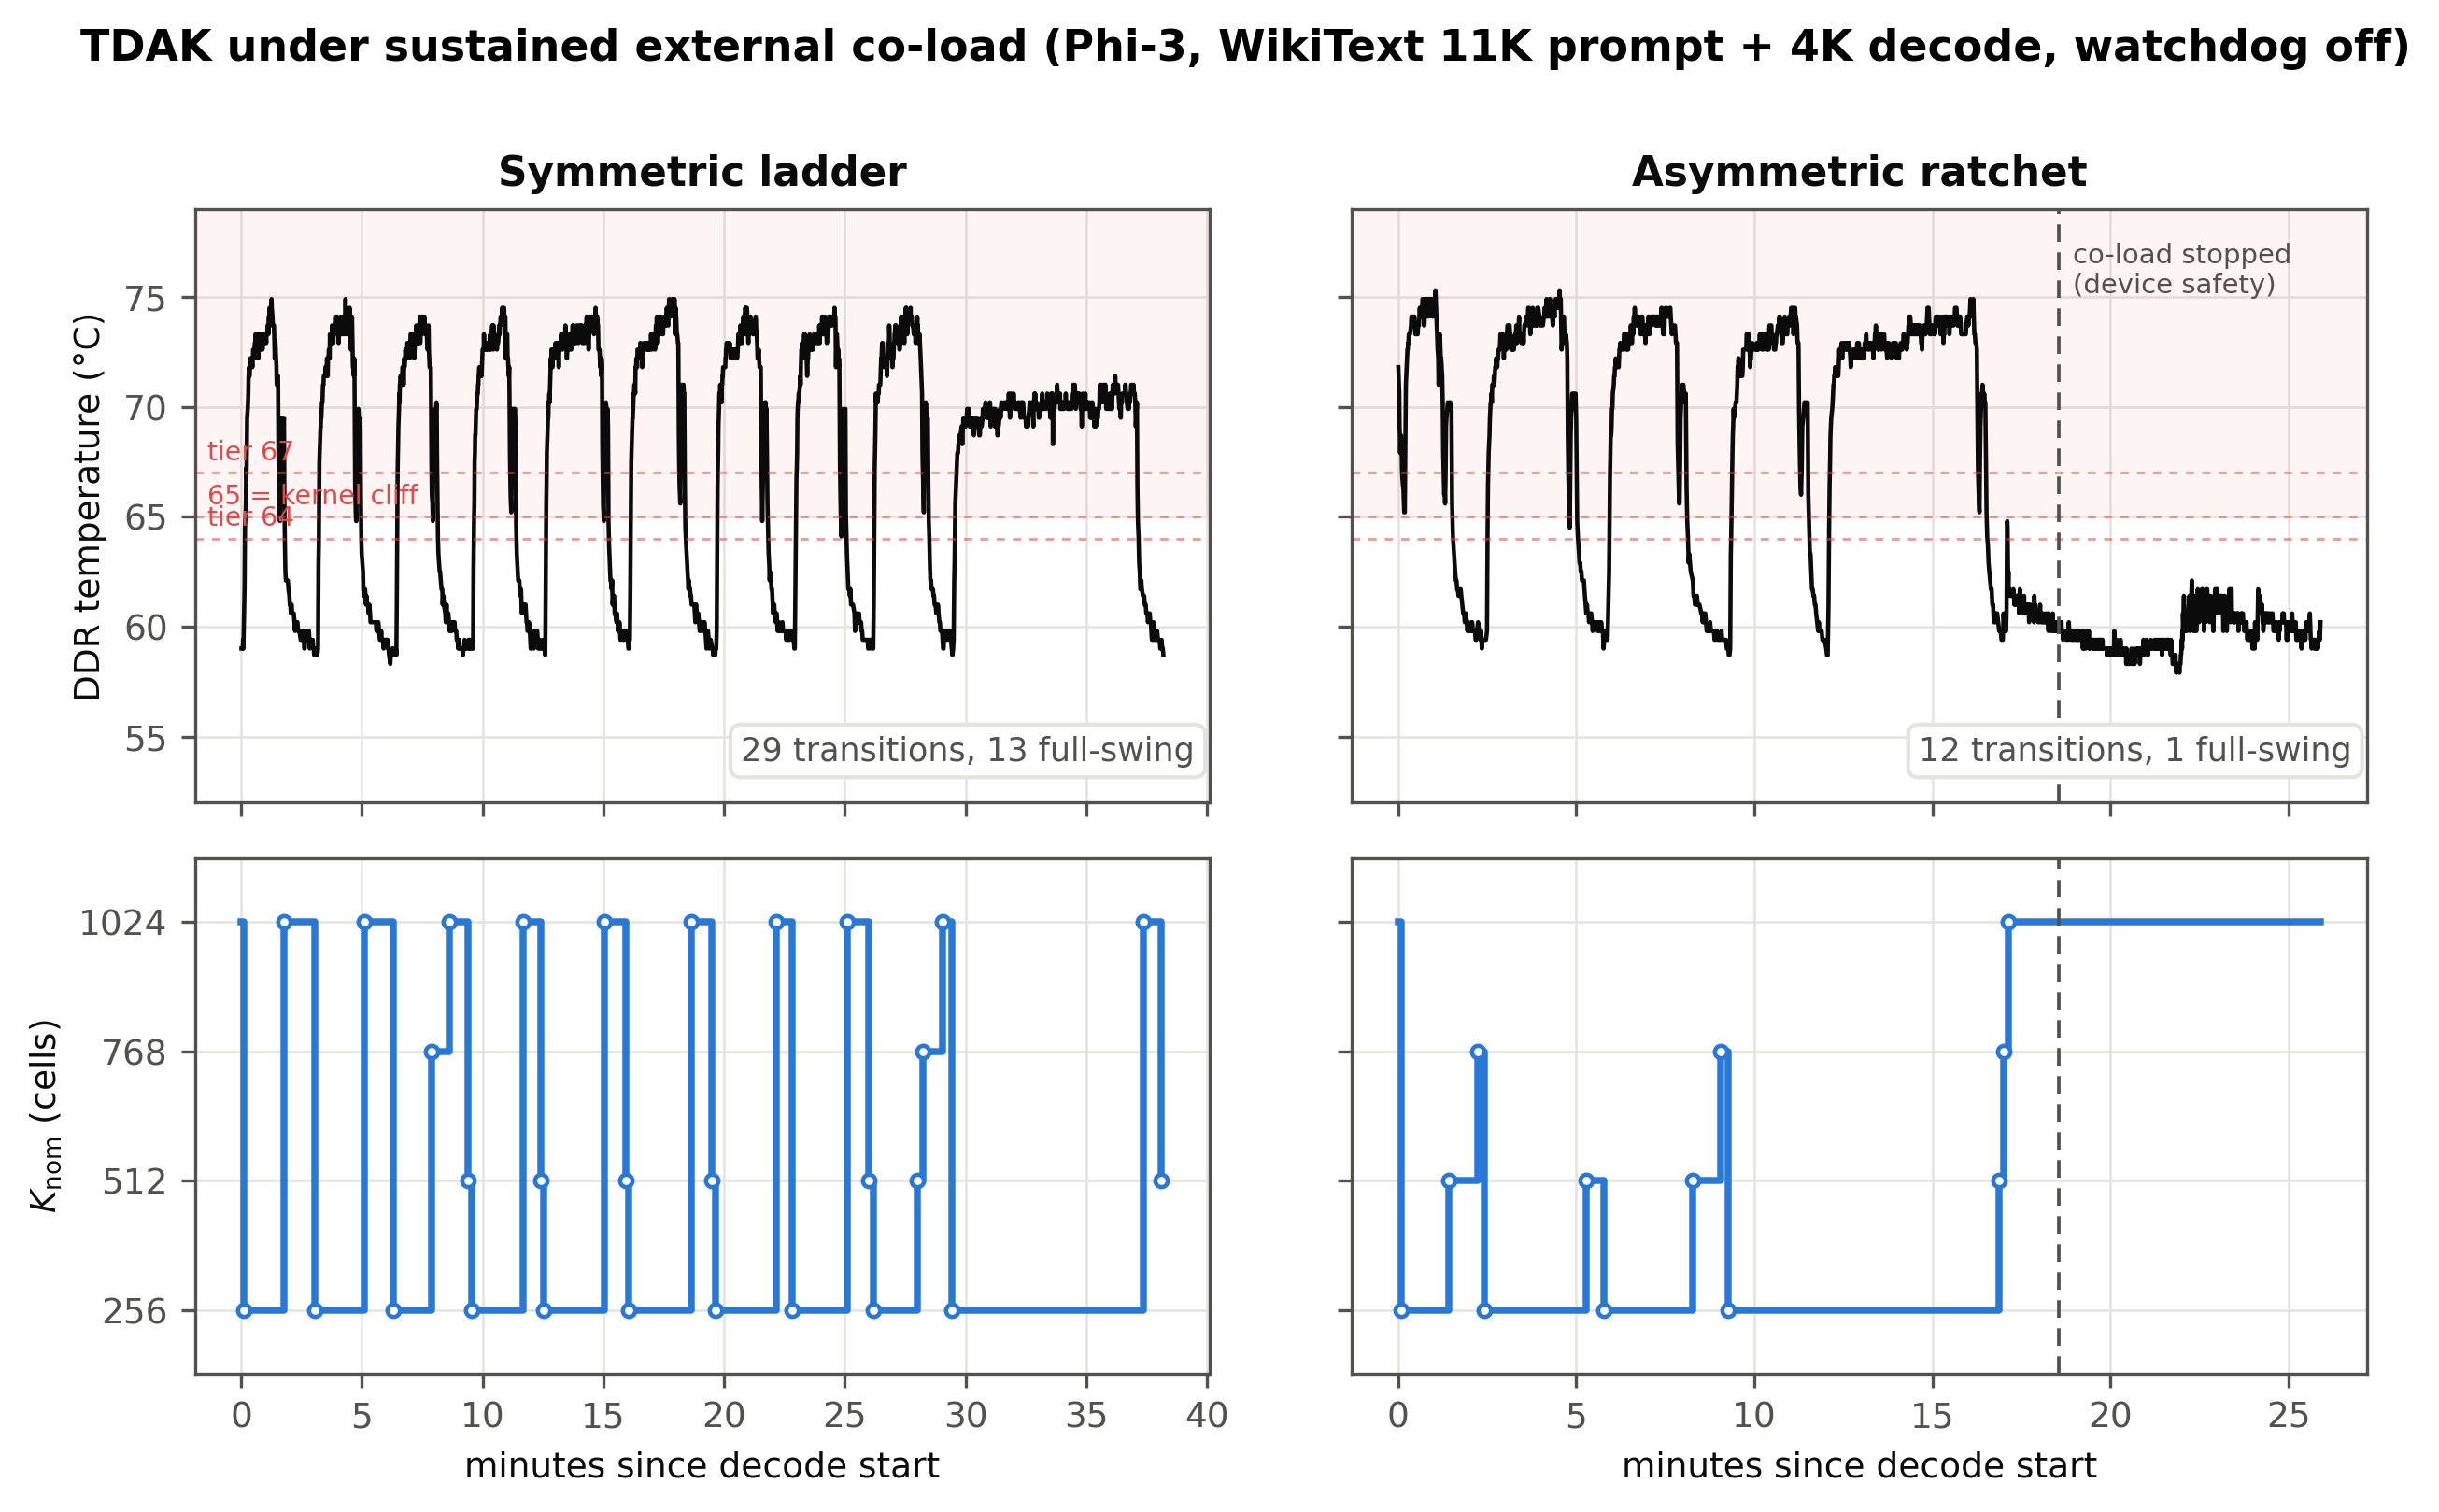
\includegraphics[width=0.9\textwidth]{figures/fig_tdak_trace.png}
\caption{\textbf{Controller traces under sustained co-load: the symmetric ladder oscillates; the ratchet does not.} Both panels run the \emph{same} TDAK thermal loop; they differ only in how $K$ may move. The \textbf{symmetric ladder} sets $K$ to whichever tier the current DDR reading falls in, moving \emph{freely up and down} the four rungs $\{256,512,768,1024\}$. The \textbf{asymmetric ratchet} steps $K$ \emph{down immediately} when hot but recovers \emph{up} only one tier at a time and only after DDR cools $\ge$1\,\textdegree C below the tier threshold --- like a mechanical ratchet, easy one way, resistant the other. Aligned panels per arm (top: DDR temperature with the 64/65/67\,\textdegree C tiers; bottom: the $K_\mathrm{nom}$ staircase the controller commanded; markers are transitions). \emph{Left, symmetric}: 29 transitions, 13 full $1024{\leftrightarrow}256$ swings --- each recovery to $K{=}1024$ visibly ignites the next DDR pulse to $\sim$75\,\textdegree C. \emph{Right, ratchet}: 12 transitions, one full swing; small one-tier recoveries; identical PPL at $+47\%$ throughput and $-23\%$ energy (Table~\ref{tab:tdak-ratchet}). The late climb back to $K{=}1024$ (right, $\sim$17\,min) is the eager-recovery artifact of the 1\,\textdegree C hysteresis --- the measured motivation for a dwell-time on recovery. Dashed vertical line: external co-load stopped early for device safety; metrics in the table use the co-load window only.}
\label{fig:tdak-trace}
\end{figure*}






%% ===== 16K 3-model campaign (tab:master) + deep-dive paragraphs moved from
%% HotMobile 2026-07-18 for the full-system version. Rewire refs as needed. =====

\paragraph{Phone 3$\times$3 — what the rows show.}
On Phi-3 (the most thermally-stressed model) $\mu$KV adapt holds DDR at 54.8\,\textdegree C (10\,\textdegree C cooler than AdaKV's 64.8 which approaches the cliff) and finishes the same 2048-token decode in 1883\,s vs vanilla's 3061\,s and AdaKV's 3228\,s (Table~\ref{tab:master}). The watchdog fires three preemptive tier transitions on the PMIC sensor (46\,\textdegree C $\to$ 47\,\textdegree C $\to$ 49\,\textdegree C) at $t{=}891/1363/1822$\,s, ratcheting the cap from 1632 $\to$ 1497 $\to$ 1267 $\to$ 883\,MHz one-way --- visible as a clean step trajectory in the NIAH sweep alongside the underlying DVFS bursts. Energy through the USB rail (clean V$\cdot$I integration, charging held OFF throughout each cell) gives \textbf{1281\,mWh for $\mu$KV vs 2230\,mWh vanilla / 2692\,mWh AdaKV} on Phi-3 (Table~\ref{tab:master}) --- $\mu$KV nearly halves system energy at $3.6\times$ vanilla throughput. The pattern holds on Llama-3.2-1B (\textbf{440--447 vs 635 vs 654}\,mWh) and gemma-2-2b (\textbf{839--856 vs 1342 vs 1381}\,mWh): $\mu$KV is always the fastest and the lowest-energy (Table~\ref{tab:master}). On quality, AdaKV wins PPL on Llama-1B and Gemma-2B (1.082 / 1.422) while $\mu$KV's saturated $\alpha_a{=}0.95$ over-allocates anchors for smaller models (1.379 / 1.751); the mass-based $\alpha_a$ deployed in Sec.~\ref{sec:eval-tdak} re-balances toward recent for these regimes (0.73--0.84 range across models, the mass-$\alpha_a$ ablation) and is expected to close this gap on a follow-on sweep.


\paragraph{Master-table headlines.}
On GPU 16K-decode, $\mu$KV-adaptive is the fastest of all three policies for every model (1.18--5.32$\times$ over AdaKV; 1.18--1.88$\times$ over vanilla), but on PPL Phi-3's old $\alpha_a{=}0.95$ saturation is visible (3.61 vs vanilla 2.83) --- the motivation for the mass-based $\alpha_a$ we deploy and validate in Sec.~\ref{sec:eval-tdak}. On LongBench QA, $\mu$KV's quality vs AdaKV/vanilla flips per (model, task): Phi-3 wins both, Llama-1B and Gemma-2B lose under the saturated $\alpha_a$. On phone, the result that matters most is the bottom three rows: $\mu$KV's two corners are 3.4$\times$--4.8$\times$ faster than vanilla on the same workload, hold DDR 8--10\,\textdegree C below the cliff vanilla crosses, and use less than half the memory at the chat corner.


\paragraph{Attributing the composite win to individual controllers.} The Phi-3 vanilla-to-$\mu$KV delta ($1.05 \to 3.76$\,tps; $2230 \to 1755$\,mWh; $79.1 \to 64.2\,^\circ$C peak CPU; Table~\ref{tab:master}) is a composite outcome, not a single controller's effect. Decomposing across the the budget ladder--the cache-budget controller stack using only measurements in this paper: (a) the q8\_0 cache q8\_0 K quantization removes roughly $43\,\%$ of the K-side DRAM read per step at zero PPL cost (Sec.~\ref{sec:design}); (b) per-head gate plus anchor selection cap the resident cache at $K_\text{nom}$ regardless of prompt length --- the mechanism that produces the $9589 \to 639$ attended-cell drop shown in Figs.~
ef{fig:main-results}--
ef{fig:thermal-trace}; (c) compaction step moves decode onto the FA-on path, converting the previous two savings into a wall-time reduction that Eq.~\eqref{eq:step-cost} predicts and Table~\ref{tab:master} confirms ($3061 \to 1934$\,s on Phi-3); (d) watchdog contributes the 176 tier transitions on the sustained-decode configuration that keep the CPU cluster off the kernel cliff (Sec.~\ref{sec:eval-thermal}). A clean per-controller cumulative ablation (add the budget ladder, +the per-head gate, $\ldots$, +the cache-budget controller) is future work: our current sweep budget was spent on the 3-model $\times$ 8-policy master grid; the ablation requires re-running six intermediate stack configurations end-to-end.


\paragraph{Honest reframing of the cache-thermal causality (data finding).} A natural reading of the 16K-decode results is ``smaller cache $\to$ less DDR bandwidth $\to$ cooler DDR.'' The data does not support that simple causation. AdaKV's attended cache is 21\,\% \emph{smaller} than vanilla's at end-of-decode (7554 vs 9590 attended cells), yet its peak DDR temperature is \emph{higher} (64.8 vs 57.5\,\textdegree C) and its total system energy (USB rail integration) is \emph{higher} (2692 vs 2230\,mWh, Table~\ref{tab:master}). The driver is the attention kernel: AdaKV runs FA-off during prefill plus a per-head max-pool selection that touches $\sim$30\,MB of DDR per layer; that score-capture machinery generates more DRAM traffic than vanilla's full-cache FA-on attention, despite holding fewer attended positions. Cache size is one of several factors; the dominant driver in this workload class is the FA kernel choice. $\mu$KV wins on DDR temperature and energy because (i) its q8\_0 K cache halves the K-side bytes per attention pass, (ii) it runs FA-on through decode (via the compaction step), and (iii) its the eviction step decode-time eviction holds attended cells at $\le K$ throughout. Regardless, cross-policy thermal comparisons must account for the kernel difference.


\paragraph{Strict-cool replication (reproducibility).} To bound single-run precision we re-collected the entire Table~\ref{tab:master} workload (same $\sim$7K-prompt/2K-decode, seed 42) under a \emph{stricter} cool-gate (DDR/CPU$\le$38\,\textdegree C, skin/PMIC/battery$\le$36\,\textdegree C, no timeout fallback --- vs $<$40/$<$36 with a timeout in Table~\ref{tab:master}). Across all 24 cells, \textbf{PPL is identical} to Table~\ref{tab:master} to two decimals (seed-42 greedy decoding is deterministic; e.g.\ Phi-3 vanilla/$\mu$KV/AdaKV $=$ 2.41/1.50/1.53 in both), confirming the quality numbers are exact rather than noisy. Decode throughput moves within $\pm$15\% between protocols (mostly slightly lower under the stricter gate on Phi-3/Llama, comparable on Gemma) --- a day-to-day/thermal-history variance that we treat as the effective error bar on the one-run-per-cell systems columns. Critically, the \emph{ordering is preserved on every model}: $\mu$KV remains the fastest, coolest (DDR), and lowest-energy policy, and AdaKV remains the hottest. Per-cell energies are $V{\cdot}I$-integrated and glitch-screened; all 24 fell within the normal 0.74--1.22\,mWh/s power band (no V$\cdot$I outliers to exclude). The full 24-cell strict-cool table is in the artifact release.


\paragraph{Measurement notes for Table~\ref{tab:master}.} Cool-baseline protocol (DDR and CPU below 40\,\textdegree C, skin and battery below 36\,\textdegree C), USB charging held off for clean $V{\cdot}I$ energy, PPL on decoded text. ActKV counts unique attended positions across heads and layers; for $\mu$KV this is sink plus anchor plus recent from the dispatcher, for baselines the prompt minus prefill evictions. Baselines run as published; $\mu$KV-mass is the recommended default.


\begin{table*}[t]
\caption{Phone 16K-context decode, 8 policies on 3 models (OnePlus 15, CPU-only, 7K-token prompt $+$ 2K decode). Earlier-protocol campaign (\S\ref{sec:revised-protocol}).}
\label{tab:master}
\centering\scriptsize
\setlength{\tabcolsep}{3pt}
\begin{tabular}{l l r r r r r r r r r}
\toprule
\textbf{Model} & \textbf{Policy} & \textbf{PPL} & \textbf{tps} & \textbf{Wall (s)} & \textbf{ActKV} & \textbf{$\alpha_a$} & \textbf{RSS (MB)} & \textbf{DDR (\textdegree C)} & \textbf{CPU (\textdegree C)} & \textbf{Energy (mWh)} \\
\midrule
\multirow{8}{*}{Phi-3-mini}
 & vanilla            & 2.41 & 1.05 & 3061 & 7542 & --- & 7507 & 57.5 & 79.1 & 2230 \\
 & $\mu$KV (count)    & \good{1.50} & 3.76 & 1883 & \good{1024} & 0.95 & \good{7199} & \good{54.8} & \good{62.7} & \good{1281} \\
 & \textbf{$\mu$KV-mass} & \good{1.50} & \good{3.76} & 1934 & \good{1024} & 0.95 & 7215 & 55.6 & \good{64.2} & 1755 \\
 & AdaKV              & 1.53 & 1.13 & 3228 & 5506 & --- & 8128 & \bad{64.8} & 69.0 & 2692 \\
 & H2O                & 1.29 & 1.39 & 2658 & 7542 & --- & 7696 & 61.4 & \bad{83.3} & \bad{3540} \\
 & TOVA               & 1.66 & 1.22 & 2962 & 4628 & --- & 7581 & 63.7 & 68.2 & 2966 \\
 & TOVA-can           & \bad{6.99} & 1.06 & 3364 & 5506 & --- & 8002 & 64.5 & 68.5 & 3157 \\
 & StrLLM             & 1.41 & 1.14 & 3264 & 886 & --- & 8068 & 64.8 & 69.0 & 3066 \\
\midrule
\multirow{8}{*}{Llama-3.2-1B}
 & vanilla            & 1.16 & 4.87 & 661 & 6401 & --- & 1338 & 56.7 & \bad{86.1} & 635 \\
 & $\mu$KV (count)    & 1.38 & 16.29 & \good{401} & \good{1024} & 0.95 & \good{1298} & 54.0 & \good{65.4} & \good{447} \\
 & \textbf{$\mu$KV-mass} & 1.38 & \good{17.73} & \good{387} & \good{1024} & 0.84 & \good{1298} & 54.4 & 65.8 & \good{440} \\
 & AdaKV              & \good{1.08} & 5.90 & 634 & 4554 & --- & 1422 & 51.7 & 60.7 & 654 \\
 & H2O                & 1.14 & 5.52 & 658 & 3335 & --- & 1470 & 50.2 & 59.6 & 694 \\
 & TOVA               & 1.31 & 5.70 & 646 & 3621 & --- & 1422 & \bad{64.8} & \bad{85.3} & 693 \\
 & TOVA-can           & \bad{8.55} & 5.18 & 682 & 4554 & --- & 1423 & 54.8 & 73.3 & 693 \\
 & StrLLM             & 1.30 & 6.09 & 623 & 769 & --- & 1422 & 51.3 & 60.0 & 638 \\
\midrule
\multirow{8}{*}{Gemma-2-2B}
 & vanilla            & 1.21 & 3.35 & 1147 & 6382 & --- & 3347 & 59.8 & 65.0 & 1342 \\
 & $\mu$KV (count)    & 1.75 & 7.17 & 884 & \good{1024} & 0.94 & \good{3020} & \good{54.8} & 64.2 & 856 \\
 & \textbf{$\mu$KV-mass} & 1.63 & \good{7.46} & \good{861} & \good{1024} & 0.87 & \good{3020} & 55.6 & 66.2 & \good{839} \\
 & AdaKV              & 1.42 & 2.69 & 1368 & 4955 & --- & 3417 & 55.6 & \good{61.1} & 1381 \\
 & H2O                & 1.40 & 2.70 & 1347 & 6382 & --- & 3494 & 54.8 & 61.5 & 1348 \\
 & TOVA               & 1.38 & 2.66 & 1369 & 4454 & --- & 3417 & 54.4 & \bad{83.0} & 1332 \\
 & TOVA-can           & \bad{5.27} & 2.36 & 1476 & 4955 & --- & 3417 & 55.2 & 76.0 & 1371 \\
 & StrLLM             & 1.26 & 2.65 & 1380 & 1006 & --- & 3416 & 54.8 & 61.5 & 1334 \\
\bottomrule
\end{tabular}
\end{table*}



%% ablation-detail paragraphs moved from HotMobile 2026-07-18

\paragraph{Why mass-$\alpha_a$ over count-$\alpha_a$.} The dispatcher started life as a binary argmax-count metric: ``does each head's peak sit outside the recent window?'', averaged over $(l, h)$ pairs. On any response-generation workload, almost every head's argmax sits on the system prompt or buried context, so the count saturates and $\alpha_a$ clamps at $0.95$ regardless of prompt type. The mass-based version (used throughout this paper) weights by actual attention mass rather than binary peak position, and varies smoothly per prompt: short chat $\alpha_a \approx 0.62$--$0.78$, medium QA $\approx 0.78$--$0.92$, long retrieval $\approx 0.81$--$0.91$. Compute cost is identical (the same column-mean reduction anchor selection already needs); the only additional state is one scalar partition sum.


\paragraph{Why smaller models want lower $\alpha_a$.} Gemma-2B and Llama-3.2-1B consistently produce lower $\alpha_a$ than Phi-3 on the same prompt class. Empirically (\S\ref{tab:master-wikitext}) these are also the models where the old argmax-count metric ($\alpha_a{=}0.95$ everywhere) hurt LongBench F1 versus AdaKV. The mass-based variant gives them appropriate recent budget --- e.g., gemma-2b on short chat allocates $192$ of $508$ non-sink slots to the recent window vs the binary-count's $25$, restoring local coherence without changing $K$.

\begin{algorithm}[t]
\caption{$\mu$KV prefill (controllers the per-head gate, anchor selection, the eviction step)}
\label{alg:prefill}
\begin{algorithmic}[1]
\Require prompt $X$, budgets $K_{\text{nom}}, n_{\text{sink}}{=}4, n_{\text{anchor}}{=}32$
\Ensure decode-ready FA-on context $\mathcal{C}_B$, cache $\le K_{\text{nom}}$
\State Build $\mathcal{C}_A$: \texttt{flash\_attn}=false, K=q8\_0, V=f16
\State Prefill; read $A_i \gets \mathrm{softmax}(q_{\text{last}}K_i^\top)$ per head $i$
\For{each head $i$}
  \State $m_i \gets \max_p A_i^p$;\ \ $K_i \gets \mathrm{round}(K_{\text{nom}}\,\mu(m_i))$
  \State $S_i \gets \mathrm{TopK}(A_i, K_i)$ \Comment{$S_i \subset [0,n)$}
\EndFor
\State $S \gets \bigcup_i S_i$;\ \ $\bar A^p \gets \tfrac1H\sum_i A_i^p$ for $p\in S$
\State $\textsc{Anchor}\gets\mathrm{TopK}(\bar A, n_{\text{anchor}})$;\ $\textsc{Sink}\gets[0,n_{\text{sink}})$
\State $\textsc{Recent}\gets[n-(K_{\text{nom}}-n_{\text{sink}}-n_{\text{anchor}}),\,n)$
\State $S_{\text{keep}}\gets\textsc{Sink}\cup\textsc{Anchor}\cup\textsc{Recent}$
\State \textsc{seq\_rm}($\mathcal{C}_A$, positions $\notin S_{\text{keep}}$)
\State buf $\gets$ \texttt{state\_seq\_get\_data}($\mathcal{C}_A$)
\State Build $\mathcal{C}_B$: \texttt{flash\_attn}=true; \texttt{state\_seq\_set\_data}($\mathcal{C}_B$, buf)
\State Warm-up decode call to populate \texttt{n\_outputs}; \Return $\mathcal{C}_B$
\end{algorithmic}
\end{algorithm}


\paragraph{Why $\mu$KV-mass is the recommended default over $\mu$KV-count.} The two variants differ only in how the dispatcher computes $\alpha_a$: count-$\alpha$ uses the binary argmax-position metric (Sec.~\ref{sec:design} the dispatcher v1), mass-$\alpha$ uses the column-mean attention partition (the dispatcher v2). On every response-generation workload measured (chat, QA, NIAH), the count-$\alpha$ saturates at 0.95 across all prompts --- it is functionally static. The mass-$\alpha$ varies smoothly per prompt: 0.62--0.78 for short chat, 0.78--0.92 for medium QA, 0.81--0.91 for long retrieval. Operationally, mass-$\alpha$ produces 40\,\% smaller active KV (250 vs 416 at 4K NIAH on Phi-3) at the same NIAH hit rate (7/7 vs 7/7), 4\,\% higher decode throughput (5.7 vs 5.5), and 2--3\,\textdegree C lower DDR temperature. The compute cost is identical (the same column-mean reduction anchor selection already requires for anchor ranking). We therefore deploy mass-$\alpha$ as the production default and retain count-$\alpha$ only as an ablation in Sec.~\ref{sec:eval-tdak}.

\end{document}
